\documentclass[twoside]{book}

% Packages required by doxygen
\usepackage{fixltx2e}
\usepackage{calc}
\usepackage{doxygen}
\usepackage[export]{adjustbox} % also loads graphicx
\usepackage{graphicx}
\usepackage[utf8]{inputenc}
\usepackage{makeidx}
\usepackage{multicol}
\usepackage{multirow}
\PassOptionsToPackage{warn}{textcomp}
\usepackage{textcomp}
\usepackage[nointegrals]{wasysym}
\usepackage[table]{xcolor}

% Font selection
\usepackage[T1]{fontenc}
\usepackage[scaled=.90]{helvet}
\usepackage{courier}
\usepackage{amssymb}
\usepackage{sectsty}
\renewcommand{\familydefault}{\sfdefault}
\allsectionsfont{%
  \fontseries{bc}\selectfont%
  \color{darkgray}%
}
\renewcommand{\DoxyLabelFont}{%
  \fontseries{bc}\selectfont%
  \color{darkgray}%
}
\newcommand{\+}{\discretionary{\mbox{\scriptsize$\hookleftarrow$}}{}{}}

% Page & text layout
\usepackage{geometry}
\geometry{%
  a4paper,%
  top=2.5cm,%
  bottom=2.5cm,%
  left=2.5cm,%
  right=2.5cm%
}
\tolerance=750
\hfuzz=15pt
\hbadness=750
\setlength{\emergencystretch}{15pt}
\setlength{\parindent}{0cm}
\setlength{\parskip}{3ex plus 2ex minus 2ex}
\makeatletter
\renewcommand{\paragraph}{%
  \@startsection{paragraph}{4}{0ex}{-1.0ex}{1.0ex}{%
    \normalfont\normalsize\bfseries\SS@parafont%
  }%
}
\renewcommand{\subparagraph}{%
  \@startsection{subparagraph}{5}{0ex}{-1.0ex}{1.0ex}{%
    \normalfont\normalsize\bfseries\SS@subparafont%
  }%
}
\makeatother

% Headers & footers
\usepackage{fancyhdr}
\pagestyle{fancyplain}
\fancyhead[LE]{\fancyplain{}{\bfseries\thepage}}
\fancyhead[CE]{\fancyplain{}{}}
\fancyhead[RE]{\fancyplain{}{\bfseries\leftmark}}
\fancyhead[LO]{\fancyplain{}{\bfseries\rightmark}}
\fancyhead[CO]{\fancyplain{}{}}
\fancyhead[RO]{\fancyplain{}{\bfseries\thepage}}
\fancyfoot[LE]{\fancyplain{}{}}
\fancyfoot[CE]{\fancyplain{}{}}
\fancyfoot[RE]{\fancyplain{}{\bfseries\scriptsize Generated by Doxygen }}
\fancyfoot[LO]{\fancyplain{}{\bfseries\scriptsize Generated by Doxygen }}
\fancyfoot[CO]{\fancyplain{}{}}
\fancyfoot[RO]{\fancyplain{}{}}
\renewcommand{\footrulewidth}{0.4pt}
\renewcommand{\chaptermark}[1]{%
  \markboth{#1}{}%
}
\renewcommand{\sectionmark}[1]{%
  \markright{\thesection\ #1}%
}

% Indices & bibliography
\usepackage{natbib}
\usepackage[titles]{tocloft}
\setcounter{tocdepth}{3}
\setcounter{secnumdepth}{5}
\makeindex

% Hyperlinks (required, but should be loaded last)
\usepackage{ifpdf}
\ifpdf
  \usepackage[pdftex,pagebackref=true]{hyperref}
\else
  \usepackage[ps2pdf,pagebackref=true]{hyperref}
\fi
\hypersetup{%
  colorlinks=true,%
  linkcolor=blue,%
  citecolor=blue,%
  unicode%
}

% Custom commands
\newcommand{\clearemptydoublepage}{%
  \newpage{\pagestyle{empty}\cleardoublepage}%
}

\usepackage{caption}
\captionsetup{labelsep=space,justification=centering,font={bf},singlelinecheck=off,skip=4pt,position=top}

%===== C O N T E N T S =====

\begin{document}

% Titlepage & ToC
\hypersetup{pageanchor=false,
             bookmarksnumbered=true,
             pdfencoding=unicode
            }
\pagenumbering{roman}
\begin{titlepage}
\vspace*{7cm}
\begin{center}%
{\Large Surrey\+D\+PK }\\
\vspace*{1cm}
{\large Generated by Doxygen 1.8.11}\\
\end{center}
\end{titlepage}
\clearemptydoublepage
\tableofcontents
\clearemptydoublepage
\pagenumbering{arabic}
\hypersetup{pageanchor=true}

%--- Begin generated contents ---
\chapter{Hierarchical Index}
\section{Class Hierarchy}
This inheritance list is sorted roughly, but not completely, alphabetically\+:\begin{DoxyCompactList}
\item \contentsline{section}{blood.\+Blood}{\pageref{classblood_1_1Blood}}{}
\item \contentsline{section}{chemical.\+Chemical}{\pageref{classchemical_1_1Chemical}}{}
\item \contentsline{section}{comp.\+Comp}{\pageref{classcomp_1_1Comp}}{}
\begin{DoxyCompactList}
\item \contentsline{section}{stracorn.\+Stra\+Corn}{\pageref{classstracorn_1_1StraCorn}}{}
\item \contentsline{section}{viaepd.\+Via\+Epd}{\pageref{classviaepd_1_1ViaEpd}}{}
\begin{DoxyCompactList}
\item \contentsline{section}{dermis.\+Dermis}{\pageref{classdermis_1_1Dermis}}{}
\end{DoxyCompactList}
\end{DoxyCompactList}
\item \contentsline{section}{config.\+Config}{\pageref{classconfig_1_1Config}}{}
\item \contentsline{section}{mesh.\+Mesh}{\pageref{classmesh_1_1Mesh}}{}
\begin{DoxyCompactList}
\item \contentsline{section}{mesh.\+Mesh\+Sink}{\pageref{classmesh_1_1MeshSink}}{}
\end{DoxyCompactList}
\item \contentsline{section}{point.\+Point}{\pageref{classpoint_1_1Point}}{}
\item \contentsline{section}{skin.\+Skin}{\pageref{classskin_1_1Skin}}{}
\begin{DoxyCompactList}
\item \contentsline{section}{skin\+\_\+setup.\+Skin\+\_\+\+Setup}{\pageref{classskin__setup_1_1Skin__Setup}}{}
\end{DoxyCompactList}
\end{DoxyCompactList}

\chapter{Class Index}
\section{Class List}
Here are the classes, structs, unions and interfaces with brief descriptions\+:\begin{DoxyCompactList}
\item\contentsline{section}{\hyperlink{classblood_1_1Blood}{blood.\+Blood} }{\pageref{classblood_1_1Blood}}{}
\item\contentsline{section}{\hyperlink{classchemical_1_1Chemical}{chemical.\+Chemical} }{\pageref{classchemical_1_1Chemical}}{}
\item\contentsline{section}{\hyperlink{classcomp_1_1Comp}{comp.\+Comp} }{\pageref{classcomp_1_1Comp}}{}
\item\contentsline{section}{\hyperlink{classconfig_1_1Config}{config.\+Config} }{\pageref{classconfig_1_1Config}}{}
\item\contentsline{section}{\hyperlink{classdermis_1_1Dermis}{dermis.\+Dermis} }{\pageref{classdermis_1_1Dermis}}{}
\item\contentsline{section}{\hyperlink{classmesh_1_1Mesh}{mesh.\+Mesh} }{\pageref{classmesh_1_1Mesh}}{}
\item\contentsline{section}{\hyperlink{classmesh_1_1MeshSink}{mesh.\+Mesh\+Sink} }{\pageref{classmesh_1_1MeshSink}}{}
\item\contentsline{section}{\hyperlink{classpoint_1_1Point}{point.\+Point} }{\pageref{classpoint_1_1Point}}{}
\item\contentsline{section}{\hyperlink{classskin_1_1Skin}{skin.\+Skin} }{\pageref{classskin_1_1Skin}}{}
\item\contentsline{section}{\hyperlink{classskin__setup_1_1Skin__Setup}{skin\+\_\+setup.\+Skin\+\_\+\+Setup} }{\pageref{classskin__setup_1_1Skin__Setup}}{}
\item\contentsline{section}{\hyperlink{classstracorn_1_1StraCorn}{stracorn.\+Stra\+Corn} }{\pageref{classstracorn_1_1StraCorn}}{}
\item\contentsline{section}{\hyperlink{classviaepd_1_1ViaEpd}{viaepd.\+Via\+Epd} }{\pageref{classviaepd_1_1ViaEpd}}{}
\end{DoxyCompactList}

\chapter{Class Documentation}
\hypertarget{classblood_1_1Blood}{}\section{blood.\+Blood Class Reference}
\label{classblood_1_1Blood}\index{blood.\+Blood@{blood.\+Blood}}
\subsection*{Public Member Functions}
\begin{DoxyCompactItemize}
\item 
def \hyperlink{classblood_1_1Blood_ace3e6d188e7983ec085d19f6920356cb}{\+\_\+\+\_\+init\+\_\+\+\_\+} (self, frac\+\_\+unbound, k\+\_\+clear, body\+\_\+mass=70, gender=\textquotesingle{}M\textquotesingle{})
\item 
def \hyperlink{classblood_1_1Blood_ac205ec72682730e1ddb3db838b43ecbd}{update\+Mass\+In\+Out\+Dermis} (self, mass\+In, mass\+Out, factor)
\begin{DoxyCompactList}\small\item\em (S\+T\+A\+RT OF) Class methods dealing with O\+DE computation \#\#\# \end{DoxyCompactList}\item 
def {\bfseries comp\+O\+D\+Edydt} (self, t, y, args=None)\hypertarget{classblood_1_1Blood_a39dfef20f3ac35b314d0c878e441f7a3}{}\label{classblood_1_1Blood_a39dfef20f3ac35b314d0c878e441f7a3}

\item 
def \hyperlink{classblood_1_1Blood_ad45ed3384aba6fb7e0e37648abaaf848}{set\+Mesh\+Conc\+\_\+all} (self, conc)\hypertarget{classblood_1_1Blood_ad45ed3384aba6fb7e0e37648abaaf848}{}\label{classblood_1_1Blood_ad45ed3384aba6fb7e0e37648abaaf848}

\begin{DoxyCompactList}\small\item\em (E\+ND OF) Class methods dealing with O\+DE computation \#\#\# \end{DoxyCompactList}\item 
def {\bfseries get\+Mesh\+Conc\+\_\+all} (self)\hypertarget{classblood_1_1Blood_a7b0fe3d5f68820b0371e76254a681443}{}\label{classblood_1_1Blood_a7b0fe3d5f68820b0371e76254a681443}

\item 
def \hyperlink{classblood_1_1Blood_a8814bc863db2657dbdd487f7feab6fab}{save\+Conc} (self, b\+\_\+1st\+\_\+time, fn)
\end{DoxyCompactItemize}
\subsection*{Public Attributes}
\begin{DoxyCompactItemize}
\item 
{\bfseries flow\+\_\+capil}\hypertarget{classblood_1_1Blood_a55ca5ca2d12e400f38efd428d4437e1b}{}\label{classblood_1_1Blood_a55ca5ca2d12e400f38efd428d4437e1b}

\item 
{\bfseries vol\+\_\+blood\+\_\+body}\hypertarget{classblood_1_1Blood_a07a75e187271c945646b1f96b6ac52e3}{}\label{classblood_1_1Blood_a07a75e187271c945646b1f96b6ac52e3}

\item 
{\bfseries conc}\hypertarget{classblood_1_1Blood_aa16b37eeb54140ebe61de58aabdf4a3d}{}\label{classblood_1_1Blood_aa16b37eeb54140ebe61de58aabdf4a3d}

\item 
{\bfseries k\+\_\+clear}\hypertarget{classblood_1_1Blood_a7832720868cc3139a87c664e312776ac}{}\label{classblood_1_1Blood_a7832720868cc3139a87c664e312776ac}

\item 
{\bfseries f\+\_\+unbound}\hypertarget{classblood_1_1Blood_ae27b72aee2decce7ec0067c2713c6a2b}{}\label{classblood_1_1Blood_ae27b72aee2decce7ec0067c2713c6a2b}

\item 
{\bfseries conc\+\_\+sink}\hypertarget{classblood_1_1Blood_a15dcf816e085edecf6e9e2f45b45b769}{}\label{classblood_1_1Blood_a15dcf816e085edecf6e9e2f45b45b769}

\item 
{\bfseries vol\+\_\+sink}\hypertarget{classblood_1_1Blood_aff02d25262daa67087a7c9072893c643}{}\label{classblood_1_1Blood_aff02d25262daa67087a7c9072893c643}

\item 
{\bfseries dim}\hypertarget{classblood_1_1Blood_a20e58b6fa8b5b3ac8edae03eb0787b8a}{}\label{classblood_1_1Blood_a20e58b6fa8b5b3ac8edae03eb0787b8a}

\item 
{\bfseries mass\+\_\+into\+\_\+dermis}\hypertarget{classblood_1_1Blood_a7f4a0a55fc889201a8587159180ee5c2}{}\label{classblood_1_1Blood_a7f4a0a55fc889201a8587159180ee5c2}

\item 
{\bfseries mass\+\_\+outfrom\+\_\+dermis}\hypertarget{classblood_1_1Blood_aafbc501fd60a1296f3df0aca7954fded}{}\label{classblood_1_1Blood_aafbc501fd60a1296f3df0aca7954fded}

\end{DoxyCompactItemize}


\subsection{Detailed Description}
\begin{DoxyVerb}\end{DoxyVerb}
 

Definition at line 16 of file blood.\+py.



\subsection{Constructor \& Destructor Documentation}
\index{blood\+::\+Blood@{blood\+::\+Blood}!\+\_\+\+\_\+init\+\_\+\+\_\+@{\+\_\+\+\_\+init\+\_\+\+\_\+}}
\index{\+\_\+\+\_\+init\+\_\+\+\_\+@{\+\_\+\+\_\+init\+\_\+\+\_\+}!blood\+::\+Blood@{blood\+::\+Blood}}
\subsubsection[{\texorpdfstring{\+\_\+\+\_\+init\+\_\+\+\_\+(self, frac\+\_\+unbound, k\+\_\+clear, body\+\_\+mass=70, gender=\textquotesingle{}\+M\textquotesingle{})}{__init__(self, frac_unbound, k_clear, body_mass=70, gender='M')}}]{\setlength{\rightskip}{0pt plus 5cm}def blood.\+Blood.\+\_\+\+\_\+init\+\_\+\+\_\+ (
\begin{DoxyParamCaption}
\item[{}]{self, }
\item[{}]{frac\+\_\+unbound, }
\item[{}]{k\+\_\+clear, }
\item[{}]{body\+\_\+mass = {\ttfamily 70}, }
\item[{}]{gender = {\ttfamily \textquotesingle{}M\textquotesingle{}}}
\end{DoxyParamCaption}
)}\hypertarget{classblood_1_1Blood_ace3e6d188e7983ec085d19f6920356cb}{}\label{classblood_1_1Blood_ace3e6d188e7983ec085d19f6920356cb}
\begin{DoxyVerb}\end{DoxyVerb}
 

Definition at line 18 of file blood.\+py.



\subsection{Member Function Documentation}
\index{blood\+::\+Blood@{blood\+::\+Blood}!save\+Conc@{save\+Conc}}
\index{save\+Conc@{save\+Conc}!blood\+::\+Blood@{blood\+::\+Blood}}
\subsubsection[{\texorpdfstring{save\+Conc(self, b\+\_\+1st\+\_\+time, fn)}{saveConc(self, b_1st_time, fn)}}]{\setlength{\rightskip}{0pt plus 5cm}def blood.\+Blood.\+save\+Conc (
\begin{DoxyParamCaption}
\item[{}]{self, }
\item[{}]{b\+\_\+1st\+\_\+time, }
\item[{}]{fn}
\end{DoxyParamCaption}
)}\hypertarget{classblood_1_1Blood_a8814bc863db2657dbdd487f7feab6fab}{}\label{classblood_1_1Blood_a8814bc863db2657dbdd487f7feab6fab}
\begin{DoxyVerb}Save concentrations to file
Args: b_1st_time -- if True, write to a new file; otherwise append to the existing file
\end{DoxyVerb}
 

Definition at line 76 of file blood.\+py.

\index{blood\+::\+Blood@{blood\+::\+Blood}!update\+Mass\+In\+Out\+Dermis@{update\+Mass\+In\+Out\+Dermis}}
\index{update\+Mass\+In\+Out\+Dermis@{update\+Mass\+In\+Out\+Dermis}!blood\+::\+Blood@{blood\+::\+Blood}}
\subsubsection[{\texorpdfstring{update\+Mass\+In\+Out\+Dermis(self, mass\+In, mass\+Out, factor)}{updateMassInOutDermis(self, massIn, massOut, factor)}}]{\setlength{\rightskip}{0pt plus 5cm}def blood.\+Blood.\+update\+Mass\+In\+Out\+Dermis (
\begin{DoxyParamCaption}
\item[{}]{self, }
\item[{}]{mass\+In, }
\item[{}]{mass\+Out, }
\item[{}]{factor}
\end{DoxyParamCaption}
)}\hypertarget{classblood_1_1Blood_ac205ec72682730e1ddb3db838b43ecbd}{}\label{classblood_1_1Blood_ac205ec72682730e1ddb3db838b43ecbd}


(S\+T\+A\+RT OF) Class methods dealing with O\+DE computation \#\#\# 

\begin{DoxyVerb}This function will be called after calculations in dermis
\end{DoxyVerb}
 

Definition at line 56 of file blood.\+py.



The documentation for this class was generated from the following file\+:\begin{DoxyCompactItemize}
\item 
blood.\+py\end{DoxyCompactItemize}

\hypertarget{classchemical_1_1Chemical}{}\section{chemical.\+Chemical Class Reference}
\label{classchemical_1_1Chemical}\index{chemical.\+Chemical@{chemical.\+Chemical}}
\subsection*{Public Member Functions}
\begin{DoxyCompactItemize}
\item 
def {\bfseries \+\_\+\+\_\+init\+\_\+\+\_\+} (self, mw, K\+\_\+ow, p\+Ka, frac\+\_\+non\+\_\+ion=None, frac\+\_\+unbound=None, acid\+\_\+base=None)\hypertarget{classchemical_1_1Chemical_a217516c99fbf0e2788782d27a261ec89}{}\label{classchemical_1_1Chemical_a217516c99fbf0e2788782d27a261ec89}

\item 
def \hyperlink{classchemical_1_1Chemical_a1aecc1f2e21b20636f65d45b3787f500}{\+\_\+\+\_\+init\+\_\+\+\_\+} (self, conf)
\item 
def \hyperlink{classchemical_1_1Chemical_a3633520af63f8eb799a8f0de381422e0}{comp\+Ion} (self)
\item 
def \hyperlink{classchemical_1_1Chemical_af738fbeec1e013883784f479ffa19852}{comp\+Binding} (self)
\end{DoxyCompactItemize}
\subsection*{Public Attributes}
\begin{DoxyCompactItemize}
\item 
{\bfseries mw}\hypertarget{classchemical_1_1Chemical_a71ef6f9ef7c34b7d5e277f6d65abaf84}{}\label{classchemical_1_1Chemical_a71ef6f9ef7c34b7d5e277f6d65abaf84}

\item 
{\bfseries r\+\_\+s}\hypertarget{classchemical_1_1Chemical_ad88241754d8905cb6ad5f92559cca73c}{}\label{classchemical_1_1Chemical_ad88241754d8905cb6ad5f92559cca73c}

\item 
{\bfseries K\+\_\+ow}\hypertarget{classchemical_1_1Chemical_a6d49dd119167d150d31462c9ed25bd34}{}\label{classchemical_1_1Chemical_a6d49dd119167d150d31462c9ed25bd34}

\item 
{\bfseries p\+Ka}\hypertarget{classchemical_1_1Chemical_a691d7f84f5ede16356517613adddb3d6}{}\label{classchemical_1_1Chemical_a691d7f84f5ede16356517613adddb3d6}

\item 
{\bfseries acid\+\_\+base}\hypertarget{classchemical_1_1Chemical_a0529584b85dd64b2eeb6bd9744356391}{}\label{classchemical_1_1Chemical_a0529584b85dd64b2eeb6bd9744356391}

\item 
{\bfseries frac\+\_\+non\+\_\+ion}\hypertarget{classchemical_1_1Chemical_a93543fa4cdf7d328201647ae4886ceda}{}\label{classchemical_1_1Chemical_a93543fa4cdf7d328201647ae4886ceda}

\item 
{\bfseries frac\+\_\+unbound}\hypertarget{classchemical_1_1Chemical_a6d8076f1203590f6591b98edd701898f}{}\label{classchemical_1_1Chemical_a6d8076f1203590f6591b98edd701898f}

\end{DoxyCompactItemize}


\subsection{Detailed Description}
\begin{DoxyVerb}Class definition for Chemical whose mass transfer is of interest
\end{DoxyVerb}
 

Definition at line 9 of file chemical.\+py.



\subsection{Constructor \& Destructor Documentation}
\index{chemical\+::\+Chemical@{chemical\+::\+Chemical}!\+\_\+\+\_\+init\+\_\+\+\_\+@{\+\_\+\+\_\+init\+\_\+\+\_\+}}
\index{\+\_\+\+\_\+init\+\_\+\+\_\+@{\+\_\+\+\_\+init\+\_\+\+\_\+}!chemical\+::\+Chemical@{chemical\+::\+Chemical}}
\subsubsection[{\texorpdfstring{\+\_\+\+\_\+init\+\_\+\+\_\+(self, conf)}{__init__(self, conf)}}]{\setlength{\rightskip}{0pt plus 5cm}def chemical.\+Chemical.\+\_\+\+\_\+init\+\_\+\+\_\+ (
\begin{DoxyParamCaption}
\item[{}]{self, }
\item[{}]{conf}
\end{DoxyParamCaption}
)}\hypertarget{classchemical_1_1Chemical_a1aecc1f2e21b20636f65d45b3787f500}{}\label{classchemical_1_1Chemical_a1aecc1f2e21b20636f65d45b3787f500}
\begin{DoxyVerb}Initialisation by importing information from an object of the class Config
\end{DoxyVerb}
 

Definition at line 24 of file chemical.\+py.



\subsection{Member Function Documentation}
\index{chemical\+::\+Chemical@{chemical\+::\+Chemical}!comp\+Binding@{comp\+Binding}}
\index{comp\+Binding@{comp\+Binding}!chemical\+::\+Chemical@{chemical\+::\+Chemical}}
\subsubsection[{\texorpdfstring{comp\+Binding(self)}{compBinding(self)}}]{\setlength{\rightskip}{0pt plus 5cm}def chemical.\+Chemical.\+comp\+Binding (
\begin{DoxyParamCaption}
\item[{}]{self}
\end{DoxyParamCaption}
)}\hypertarget{classchemical_1_1Chemical_af738fbeec1e013883784f479ffa19852}{}\label{classchemical_1_1Chemical_af738fbeec1e013883784f479ffa19852}
\begin{DoxyVerb}Compute the fraction of unbound in a 2.7% albumin solution at pH 7.4 (frac_unbound)
Refs:  Yamazaki K, Kanaoka M (2004). Journal of Pharmaceutical Sciences, 93: 1480.
\end{DoxyVerb}
 

Definition at line 41 of file chemical.\+py.

\index{chemical\+::\+Chemical@{chemical\+::\+Chemical}!comp\+Ion@{comp\+Ion}}
\index{comp\+Ion@{comp\+Ion}!chemical\+::\+Chemical@{chemical\+::\+Chemical}}
\subsubsection[{\texorpdfstring{comp\+Ion(self)}{compIon(self)}}]{\setlength{\rightskip}{0pt plus 5cm}def chemical.\+Chemical.\+comp\+Ion (
\begin{DoxyParamCaption}
\item[{}]{self}
\end{DoxyParamCaption}
)}\hypertarget{classchemical_1_1Chemical_a3633520af63f8eb799a8f0de381422e0}{}\label{classchemical_1_1Chemical_a3633520af63f8eb799a8f0de381422e0}
\begin{DoxyVerb}Compute the fraction of solute non-ionised at pH 7.4 (frac_non_ion) 
Refs: Florence AT, Attwood D (2006). Physicochemical Principles of Pharmacy, Pharmaceutical Press, London, p. 77.
\end{DoxyVerb}
 

Definition at line 30 of file chemical.\+py.



The documentation for this class was generated from the following file\+:\begin{DoxyCompactItemize}
\item 
chemical.\+py\end{DoxyCompactItemize}

\hypertarget{classcomp_1_1Comp}{}\section{comp.\+Comp Class Reference}
\label{classcomp_1_1Comp}\index{comp.\+Comp@{comp.\+Comp}}
Inheritance diagram for comp.\+Comp\+:\begin{figure}[H]
\begin{center}
\leavevmode
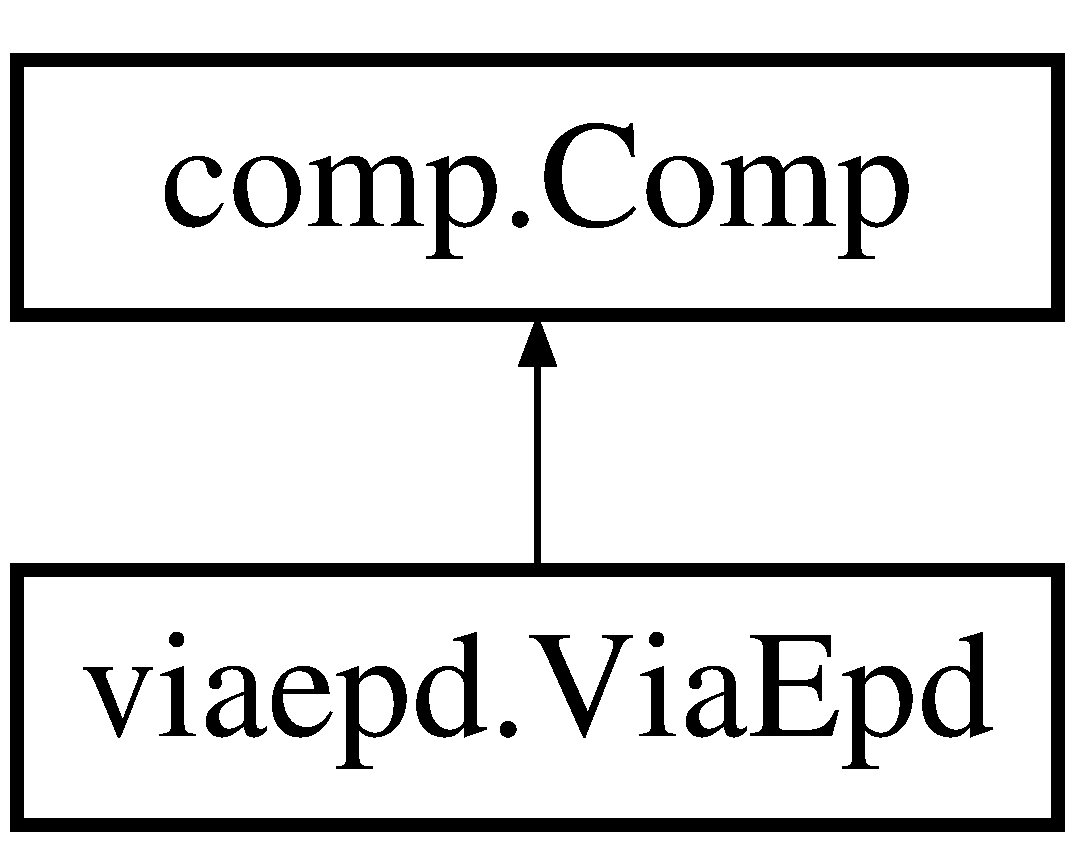
\includegraphics[height=2.000000cm]{classcomp_1_1Comp}
\end{center}
\end{figure}
\subsection*{Public Member Functions}
\begin{DoxyCompactItemize}
\item 
def \hyperlink{classcomp_1_1Comp_a041986f019d03d7fc7d2d7a400d92966}{\+\_\+\+\_\+init\+\_\+\+\_\+} (self, \hyperlink{classcomp_1_1Comp_ae00e132d485d50acaf13977284fd9051}{coord\+\_\+sys}=None, dz\+\_\+dtheta=None, bdy\+\_\+cond=None)
\item 
def {\bfseries get\+\_\+dim} (self)\hypertarget{classcomp_1_1Comp_a194c4491ee3b385837577d7c13ec78a9}{}\label{classcomp_1_1Comp_a194c4491ee3b385837577d7c13ec78a9}

\item 
def {\bfseries get\+\_\+nx} (self)\hypertarget{classcomp_1_1Comp_a4bc59e92071b7ca507e44d53433a4bf7}{}\label{classcomp_1_1Comp_a4bc59e92071b7ca507e44d53433a4bf7}

\item 
def {\bfseries get\+\_\+ny} (self)\hypertarget{classcomp_1_1Comp_aa9754974a57bbe51a9ed46a0205ae505}{}\label{classcomp_1_1Comp_aa9754974a57bbe51a9ed46a0205ae505}

\item 
def {\bfseries get\+\_\+bdy\+Cond} (self, direction)\hypertarget{classcomp_1_1Comp_a32251f4a77a6fe555508981111c6b451}{}\label{classcomp_1_1Comp_a32251f4a77a6fe555508981111c6b451}

\item 
def \hyperlink{classcomp_1_1Comp_af89f05ea9ea53f88ecfa59a503827d23}{create\+Bdy} (self, n\+Mesh\+Bdy\+Right, n\+Mesh\+Bdy\+Down)
\begin{DoxyCompactList}\small\item\em (S\+T\+A\+RT OF) Class methods dealing with boundaries \#\#\# \end{DoxyCompactList}\item 
def \hyperlink{classcomp_1_1Comp_a35ef9e925796bb10640cfe40d5f82c4b}{set\+Bdy\+Mesh} (self, mesh\+Bdy\+Right, mesh\+Bdy\+Down)
\item 
def \hyperlink{classcomp_1_1Comp_a9515ffba9a1e5a0de8542cb736e8ece4}{set\+Bdy\+Conc} (self, conc\+Bdy\+Right, conc\+Bdy\+Down)
\item 
def {\bfseries set\+Bdy\+Mass\+In\+Out\+Zero} (self)\hypertarget{classcomp_1_1Comp_a3811398d197bce2ff384b4f3610eeb0a}{}\label{classcomp_1_1Comp_a3811398d197bce2ff384b4f3610eeb0a}

\item 
def \hyperlink{classcomp_1_1Comp_a4079436132c3be952506f2652a700baa}{pass\+Bdy\+Mass\+Out} (self, bdy\+Right, bdy\+Down)
\item 
def {\bfseries set\+Mass\+In\+\_\+left} (self, mass\+In\+\_\+left)\hypertarget{classcomp_1_1Comp_a86835c18bf9c9b7ce67d0362fc2bd165}{}\label{classcomp_1_1Comp_a86835c18bf9c9b7ce67d0362fc2bd165}

\item 
def {\bfseries set\+Mass\+In\+\_\+up} (self, mass\+In\+\_\+up)\hypertarget{classcomp_1_1Comp_a704cddd08bfe38a86e5658744f33a4de}{}\label{classcomp_1_1Comp_a704cddd08bfe38a86e5658744f33a4de}

\item 
def \hyperlink{classcomp_1_1Comp_af6d700899b8a97e67233d25626554263}{comp\+Total\+Area} (self, direction)
\begin{DoxyCompactList}\small\item\em (E\+ND OF) Class methods dealing with boundaries \#\#\# \end{DoxyCompactList}\item 
def {\bfseries comp\+Total\+Volume} (self)\hypertarget{classcomp_1_1Comp_ac8ec3d15a67a816e5a42ff5facf6753b}{}\label{classcomp_1_1Comp_ac8ec3d15a67a816e5a42ff5facf6753b}

\item 
def \hyperlink{classcomp_1_1Comp_a0f93a3308637381e7342a2a7497d174d}{comp\+Mass\+Irreg\+Mesh\+Right} (self, mesh\+This, conc\+\_\+this)
\begin{DoxyCompactList}\small\item\em (E\+ND OF) Class methods dealing with geometries \#\#\# \end{DoxyCompactList}\item 
def \hyperlink{classcomp_1_1Comp_a7b78ad68606fdf55c38c3de6d5a67570}{comp\+Mass\+Irreg\+Mesh\+Down} (self, mesh\+This, conc\+\_\+this)
\item 
def \hyperlink{classcomp_1_1Comp_af33e252fda921dadb0e80c825e48e386}{comp\+O\+D\+Edydt\+\_\+diffu} (self, t, y, args=None)
\begin{DoxyCompactList}\small\item\em (E\+ND OF) Class methods dealing with geometries \#\#\# \end{DoxyCompactList}\item 
def \hyperlink{classcomp_1_1Comp_ad2c0555c16dc7b5bf639407fa44bfaf7}{display\+Mesh} (self)
\begin{DoxyCompactList}\small\item\em (E\+ND OF) Class methods dealing with O\+DE computation \#\#\# \end{DoxyCompactList}\item 
def \hyperlink{classcomp_1_1Comp_a7b8cd6483a2de95d92a0d5b4d939ca65}{get\+Total\+Mass} (self)
\item 
def \hyperlink{classcomp_1_1Comp_ac100eb9f8d55df5f9f761cbe45a58024}{get\+Mesh\+Conc} (self)
\item 
def \hyperlink{classcomp_1_1Comp_afa8ff8a057f1c9ee1ddd027b08a3160c}{set\+Mesh\+Conc} (self, conc)
\item 
def \hyperlink{classcomp_1_1Comp_ad6b532a1d5c1aa95b9a88124a5b5609d}{set\+Mesh\+Conc} (self, conc, idx\+\_\+x, idx\+\_\+y)
\item 
def \hyperlink{classcomp_1_1Comp_afe675826a85b99ab6dc5de7ed02a2e0d}{save\+Mesh\+Conc} (self, b\+\_\+1st\+\_\+time, fn)
\item 
def \hyperlink{classcomp_1_1Comp_a61ca5ccfbb7e0ee1244931e78eb5a35d}{get\+X\+Coord} (self)
\item 
def \hyperlink{classcomp_1_1Comp_ab61436b8f65a7f8c45fb554e412cdfa3}{get\+Y\+Coord} (self)
\item 
def \hyperlink{classcomp_1_1Comp_a0268c9629d4839526c1e81114adc2408}{save\+Coord} (self, fn\+\_\+x, fn\+\_\+y, fn\+\_\+suffix)
\end{DoxyCompactItemize}
\subsection*{Public Attributes}
\begin{DoxyCompactItemize}
\item 
\hyperlink{classcomp_1_1Comp_ae00e132d485d50acaf13977284fd9051}{coord\+\_\+sys}\hypertarget{classcomp_1_1Comp_ae00e132d485d50acaf13977284fd9051}{}\label{classcomp_1_1Comp_ae00e132d485d50acaf13977284fd9051}

\begin{DoxyCompactList}\small\item\em geometric parameters \#\#\# \end{DoxyCompactList}\item 
{\bfseries x\+\_\+length}\hypertarget{classcomp_1_1Comp_ab00f0017e7b9e2a1358d200872bc5d45}{}\label{classcomp_1_1Comp_ab00f0017e7b9e2a1358d200872bc5d45}

\item 
{\bfseries y\+\_\+length}\hypertarget{classcomp_1_1Comp_a238a265e564e002cb32f816e588fedda}{}\label{classcomp_1_1Comp_a238a265e564e002cb32f816e588fedda}

\item 
{\bfseries dz\+\_\+dtheta}\hypertarget{classcomp_1_1Comp_a46b24a2ad70c60858be5970dd249e42f}{}\label{classcomp_1_1Comp_a46b24a2ad70c60858be5970dd249e42f}

\item 
{\bfseries nx}\hypertarget{classcomp_1_1Comp_aa57c2e18312b3ff75ca85e5b91630c1e}{}\label{classcomp_1_1Comp_aa57c2e18312b3ff75ca85e5b91630c1e}

\item 
{\bfseries ny}\hypertarget{classcomp_1_1Comp_ac88e268c8aa6dc536ec4d91ced077193}{}\label{classcomp_1_1Comp_ac88e268c8aa6dc536ec4d91ced077193}

\item 
{\bfseries dim}\hypertarget{classcomp_1_1Comp_a5ad617a643f9f0b33d82cb7c774409d3}{}\label{classcomp_1_1Comp_a5ad617a643f9f0b33d82cb7c774409d3}

\item 
\hyperlink{classcomp_1_1Comp_a3a618fb7afb0d89e902b18620f194cbb}{n\+\_\+mesh\+Bdy\+Right}\hypertarget{classcomp_1_1Comp_a3a618fb7afb0d89e902b18620f194cbb}{}\label{classcomp_1_1Comp_a3a618fb7afb0d89e902b18620f194cbb}

\begin{DoxyCompactList}\small\item\em compartment boundary parameters \#\#\# \end{DoxyCompactList}\item 
{\bfseries n\+\_\+mesh\+Bdy\+Down}\hypertarget{classcomp_1_1Comp_a9252858541b296d523e5a44d68f9cedf}{}\label{classcomp_1_1Comp_a9252858541b296d523e5a44d68f9cedf}

\item 
{\bfseries bdy\+Cond}\hypertarget{classcomp_1_1Comp_a823a5dec18a94793a7bcf36146f09d3c}{}\label{classcomp_1_1Comp_a823a5dec18a94793a7bcf36146f09d3c}

\item 
{\bfseries mesh\+Bdy\+Right}\hypertarget{classcomp_1_1Comp_aab5f766e5680035613a8f6b2a5408ef7}{}\label{classcomp_1_1Comp_aab5f766e5680035613a8f6b2a5408ef7}

\item 
{\bfseries mesh\+Bdy\+Down}\hypertarget{classcomp_1_1Comp_af5c9999c82110bffe604c7f788c0e6d8}{}\label{classcomp_1_1Comp_af5c9999c82110bffe604c7f788c0e6d8}

\item 
{\bfseries mass\+In\+\_\+up}\hypertarget{classcomp_1_1Comp_a85fc4415f3e5515b4bb7a1af3f84c855}{}\label{classcomp_1_1Comp_a85fc4415f3e5515b4bb7a1af3f84c855}

\item 
{\bfseries mass\+In\+\_\+left}\hypertarget{classcomp_1_1Comp_a665b8775b8f6f1aac3b09b3de2e9e581}{}\label{classcomp_1_1Comp_a665b8775b8f6f1aac3b09b3de2e9e581}

\item 
{\bfseries mass\+Out\+\_\+right}\hypertarget{classcomp_1_1Comp_ac238bc0ae06b22177f0dbb5a91b64383}{}\label{classcomp_1_1Comp_ac238bc0ae06b22177f0dbb5a91b64383}

\item 
{\bfseries mass\+Out\+\_\+down}\hypertarget{classcomp_1_1Comp_a172c670a337fbebe17b368c8a9d3982b}{}\label{classcomp_1_1Comp_a172c670a337fbebe17b368c8a9d3982b}

\item 
{\bfseries mesh\+Sink}\hypertarget{classcomp_1_1Comp_a33d823aa69b18368d38c187c0757e2d7}{}\label{classcomp_1_1Comp_a33d823aa69b18368d38c187c0757e2d7}

\item 
{\bfseries meshes}\hypertarget{classcomp_1_1Comp_a26ad0c7c4e3d263bcccb68490d70619f}{}\label{classcomp_1_1Comp_a26ad0c7c4e3d263bcccb68490d70619f}

\item 
{\bfseries has\+Solid}\hypertarget{classcomp_1_1Comp_a6894ab3001bc910172c37e21856d42ea}{}\label{classcomp_1_1Comp_a6894ab3001bc910172c37e21856d42ea}

\item 
{\bfseries mass\+Solid}\hypertarget{classcomp_1_1Comp_a7641524ebe44ee401e2fc5aca2b2edfe}{}\label{classcomp_1_1Comp_a7641524ebe44ee401e2fc5aca2b2edfe}

\end{DoxyCompactItemize}


\subsection{Detailed Description}
\begin{DoxyVerb}Class definition for Comp
which are compartments for modelling dermato-pharmacokinetics.
This is the parent class that contains computational meshes.
From this class the compartments of stratum corneum, viable epidermis,
dermis, blood, hair follicle, sebum layer on top of skin, vehicle etc.
will be derived as daughter classes.\end{DoxyVerb}
 

Definition at line 11 of file comp.\+py.



\subsection{Constructor \& Destructor Documentation}
\index{comp\+::\+Comp@{comp\+::\+Comp}!\+\_\+\+\_\+init\+\_\+\+\_\+@{\+\_\+\+\_\+init\+\_\+\+\_\+}}
\index{\+\_\+\+\_\+init\+\_\+\+\_\+@{\+\_\+\+\_\+init\+\_\+\+\_\+}!comp\+::\+Comp@{comp\+::\+Comp}}
\subsubsection[{\texorpdfstring{\+\_\+\+\_\+init\+\_\+\+\_\+(self, coord\+\_\+sys=\+None, dz\+\_\+dtheta=\+None, bdy\+\_\+cond=\+None)}{__init__(self, coord_sys=None, dz_dtheta=None, bdy_cond=None)}}]{\setlength{\rightskip}{0pt plus 5cm}def comp.\+Comp.\+\_\+\+\_\+init\+\_\+\+\_\+ (
\begin{DoxyParamCaption}
\item[{}]{self, }
\item[{}]{coord\+\_\+sys = {\ttfamily None}, }
\item[{}]{dz\+\_\+dtheta = {\ttfamily None}, }
\item[{}]{bdy\+\_\+cond = {\ttfamily None}}
\end{DoxyParamCaption}
)}\hypertarget{classcomp_1_1Comp_a041986f019d03d7fc7d2d7a400d92966}{}\label{classcomp_1_1Comp_a041986f019d03d7fc7d2d7a400d92966}
\begin{DoxyVerb}Define instance variables and assign default values.
Geometric parameters will be setup at the compartment-specific initialisation
Thus here most default values are set to non-meaning values
\end{DoxyVerb}
 

Definition at line 20 of file comp.\+py.



\subsection{Member Function Documentation}
\index{comp\+::\+Comp@{comp\+::\+Comp}!comp\+Mass\+Irreg\+Mesh\+Down@{comp\+Mass\+Irreg\+Mesh\+Down}}
\index{comp\+Mass\+Irreg\+Mesh\+Down@{comp\+Mass\+Irreg\+Mesh\+Down}!comp\+::\+Comp@{comp\+::\+Comp}}
\subsubsection[{\texorpdfstring{comp\+Mass\+Irreg\+Mesh\+Down(self, mesh\+This, conc\+\_\+this)}{compMassIrregMeshDown(self, meshThis, conc_this)}}]{\setlength{\rightskip}{0pt plus 5cm}def comp.\+Comp.\+comp\+Mass\+Irreg\+Mesh\+Down (
\begin{DoxyParamCaption}
\item[{}]{self, }
\item[{}]{mesh\+This, }
\item[{}]{conc\+\_\+this}
\end{DoxyParamCaption}
)}\hypertarget{classcomp_1_1Comp_a7b78ad68606fdf55c38c3de6d5a67570}{}\label{classcomp_1_1Comp_a7b78ad68606fdf55c38c3de6d5a67570}
\begin{DoxyVerb}Compute mass transfer between meshThis and neighbouring meshes downward
whose meshing does not match exactly to meshThis, e.g. 
meshThis may interface with multiple meshess with self.meshBdyDown
\end{DoxyVerb}
 

Definition at line 241 of file comp.\+py.

\index{comp\+::\+Comp@{comp\+::\+Comp}!comp\+Mass\+Irreg\+Mesh\+Right@{comp\+Mass\+Irreg\+Mesh\+Right}}
\index{comp\+Mass\+Irreg\+Mesh\+Right@{comp\+Mass\+Irreg\+Mesh\+Right}!comp\+::\+Comp@{comp\+::\+Comp}}
\subsubsection[{\texorpdfstring{comp\+Mass\+Irreg\+Mesh\+Right(self, mesh\+This, conc\+\_\+this)}{compMassIrregMeshRight(self, meshThis, conc_this)}}]{\setlength{\rightskip}{0pt plus 5cm}def comp.\+Comp.\+comp\+Mass\+Irreg\+Mesh\+Right (
\begin{DoxyParamCaption}
\item[{}]{self, }
\item[{}]{mesh\+This, }
\item[{}]{conc\+\_\+this}
\end{DoxyParamCaption}
)}\hypertarget{classcomp_1_1Comp_a0f93a3308637381e7342a2a7497d174d}{}\label{classcomp_1_1Comp_a0f93a3308637381e7342a2a7497d174d}


(E\+ND OF) Class methods dealing with geometries \#\#\# 

(S\+T\+A\+RT OF) Class methods dealing with geometries \#\#\# \begin{DoxyVerb}Compute mass transfer between meshThis and neighbouring meshes to the right
whose meshing does not match exactly to meshThis, e.g. 
meshThis may interface with multiple meshess with self.meshBdyRight
\end{DoxyVerb}
 

Definition at line 186 of file comp.\+py.

\index{comp\+::\+Comp@{comp\+::\+Comp}!comp\+O\+D\+Edydt\+\_\+diffu@{comp\+O\+D\+Edydt\+\_\+diffu}}
\index{comp\+O\+D\+Edydt\+\_\+diffu@{comp\+O\+D\+Edydt\+\_\+diffu}!comp\+::\+Comp@{comp\+::\+Comp}}
\subsubsection[{\texorpdfstring{comp\+O\+D\+Edydt\+\_\+diffu(self, t, y, args=\+None)}{compODEdydt_diffu(self, t, y, args=None)}}]{\setlength{\rightskip}{0pt plus 5cm}def comp.\+Comp.\+comp\+O\+D\+Edydt\+\_\+diffu (
\begin{DoxyParamCaption}
\item[{}]{self, }
\item[{}]{t, }
\item[{}]{y, }
\item[{}]{args = {\ttfamily None}}
\end{DoxyParamCaption}
)}\hypertarget{classcomp_1_1Comp_af33e252fda921dadb0e80c825e48e386}{}\label{classcomp_1_1Comp_af33e252fda921dadb0e80c825e48e386}


(E\+ND OF) Class methods dealing with geometries \#\#\# 

(S\+T\+A\+RT OF) Class methods dealing with O\+DE computation \#\#\# \begin{DoxyVerb}Compute the right-hand side of the ODEs, i.e. dydt, due to diffusion
\end{DoxyVerb}
 

Definition at line 298 of file comp.\+py.

\index{comp\+::\+Comp@{comp\+::\+Comp}!comp\+Total\+Area@{comp\+Total\+Area}}
\index{comp\+Total\+Area@{comp\+Total\+Area}!comp\+::\+Comp@{comp\+::\+Comp}}
\subsubsection[{\texorpdfstring{comp\+Total\+Area(self, direction)}{compTotalArea(self, direction)}}]{\setlength{\rightskip}{0pt plus 5cm}def comp.\+Comp.\+comp\+Total\+Area (
\begin{DoxyParamCaption}
\item[{}]{self, }
\item[{}]{direction}
\end{DoxyParamCaption}
)}\hypertarget{classcomp_1_1Comp_af6d700899b8a97e67233d25626554263}{}\label{classcomp_1_1Comp_af6d700899b8a97e67233d25626554263}


(E\+ND OF) Class methods dealing with boundaries \#\#\# 

(S\+T\+A\+RT OF) Class methods dealing with geometries \#\#\# \begin{DoxyVerb}Compute self's total area to a certain direction
direction: [0] = up; [1] = left; [2] = right; [3] = down 
\end{DoxyVerb}
 

Definition at line 145 of file comp.\+py.

\index{comp\+::\+Comp@{comp\+::\+Comp}!create\+Bdy@{create\+Bdy}}
\index{create\+Bdy@{create\+Bdy}!comp\+::\+Comp@{comp\+::\+Comp}}
\subsubsection[{\texorpdfstring{create\+Bdy(self, n\+Mesh\+Bdy\+Right, n\+Mesh\+Bdy\+Down)}{createBdy(self, nMeshBdyRight, nMeshBdyDown)}}]{\setlength{\rightskip}{0pt plus 5cm}def comp.\+Comp.\+create\+Bdy (
\begin{DoxyParamCaption}
\item[{}]{self, }
\item[{}]{n\+Mesh\+Bdy\+Right, }
\item[{}]{n\+Mesh\+Bdy\+Down}
\end{DoxyParamCaption}
)}\hypertarget{classcomp_1_1Comp_af89f05ea9ea53f88ecfa59a503827d23}{}\label{classcomp_1_1Comp_af89f05ea9ea53f88ecfa59a503827d23}


(S\+T\+A\+RT OF) Class methods dealing with boundaries \#\#\# 

\begin{DoxyVerb}Create the meshes and mass arrays to hold boundary information
\end{DoxyVerb}
 

Definition at line 76 of file comp.\+py.

\index{comp\+::\+Comp@{comp\+::\+Comp}!display\+Mesh@{display\+Mesh}}
\index{display\+Mesh@{display\+Mesh}!comp\+::\+Comp@{comp\+::\+Comp}}
\subsubsection[{\texorpdfstring{display\+Mesh(self)}{displayMesh(self)}}]{\setlength{\rightskip}{0pt plus 5cm}def comp.\+Comp.\+display\+Mesh (
\begin{DoxyParamCaption}
\item[{}]{self}
\end{DoxyParamCaption}
)}\hypertarget{classcomp_1_1Comp_ad2c0555c16dc7b5bf639407fa44bfaf7}{}\label{classcomp_1_1Comp_ad2c0555c16dc7b5bf639407fa44bfaf7}


(E\+ND OF) Class methods dealing with O\+DE computation \#\#\# 

(S\+T\+A\+RT OF) Class methods dealing with I/O \#\#\# \begin{DoxyVerb}\end{DoxyVerb}
 

Definition at line 432 of file comp.\+py.

\index{comp\+::\+Comp@{comp\+::\+Comp}!get\+Mesh\+Conc@{get\+Mesh\+Conc}}
\index{get\+Mesh\+Conc@{get\+Mesh\+Conc}!comp\+::\+Comp@{comp\+::\+Comp}}
\subsubsection[{\texorpdfstring{get\+Mesh\+Conc(self)}{getMeshConc(self)}}]{\setlength{\rightskip}{0pt plus 5cm}def comp.\+Comp.\+get\+Mesh\+Conc (
\begin{DoxyParamCaption}
\item[{}]{self}
\end{DoxyParamCaption}
)}\hypertarget{classcomp_1_1Comp_ac100eb9f8d55df5f9f761cbe45a58024}{}\label{classcomp_1_1Comp_ac100eb9f8d55df5f9f761cbe45a58024}
\begin{DoxyVerb}Return the concentration from all meshes into a single numpy array
\end{DoxyVerb}
 

Definition at line 467 of file comp.\+py.

\index{comp\+::\+Comp@{comp\+::\+Comp}!get\+Total\+Mass@{get\+Total\+Mass}}
\index{get\+Total\+Mass@{get\+Total\+Mass}!comp\+::\+Comp@{comp\+::\+Comp}}
\subsubsection[{\texorpdfstring{get\+Total\+Mass(self)}{getTotalMass(self)}}]{\setlength{\rightskip}{0pt plus 5cm}def comp.\+Comp.\+get\+Total\+Mass (
\begin{DoxyParamCaption}
\item[{}]{self}
\end{DoxyParamCaption}
)}\hypertarget{classcomp_1_1Comp_a7b8cd6483a2de95d92a0d5b4d939ca65}{}\label{classcomp_1_1Comp_a7b8cd6483a2de95d92a0d5b4d939ca65}
\begin{DoxyVerb}\end{DoxyVerb}
 

Definition at line 455 of file comp.\+py.

\index{comp\+::\+Comp@{comp\+::\+Comp}!get\+X\+Coord@{get\+X\+Coord}}
\index{get\+X\+Coord@{get\+X\+Coord}!comp\+::\+Comp@{comp\+::\+Comp}}
\subsubsection[{\texorpdfstring{get\+X\+Coord(self)}{getXCoord(self)}}]{\setlength{\rightskip}{0pt plus 5cm}def comp.\+Comp.\+get\+X\+Coord (
\begin{DoxyParamCaption}
\item[{}]{self}
\end{DoxyParamCaption}
)}\hypertarget{classcomp_1_1Comp_a61ca5ccfbb7e0ee1244931e78eb5a35d}{}\label{classcomp_1_1Comp_a61ca5ccfbb7e0ee1244931e78eb5a35d}
\begin{DoxyVerb}Get x-coordinates and return a numpy array
\end{DoxyVerb}
 

Definition at line 511 of file comp.\+py.

\index{comp\+::\+Comp@{comp\+::\+Comp}!get\+Y\+Coord@{get\+Y\+Coord}}
\index{get\+Y\+Coord@{get\+Y\+Coord}!comp\+::\+Comp@{comp\+::\+Comp}}
\subsubsection[{\texorpdfstring{get\+Y\+Coord(self)}{getYCoord(self)}}]{\setlength{\rightskip}{0pt plus 5cm}def comp.\+Comp.\+get\+Y\+Coord (
\begin{DoxyParamCaption}
\item[{}]{self}
\end{DoxyParamCaption}
)}\hypertarget{classcomp_1_1Comp_ab61436b8f65a7f8c45fb554e412cdfa3}{}\label{classcomp_1_1Comp_ab61436b8f65a7f8c45fb554e412cdfa3}
\begin{DoxyVerb}Get y-coordinates and return a numpy array
\end{DoxyVerb}
 

Definition at line 523 of file comp.\+py.

\index{comp\+::\+Comp@{comp\+::\+Comp}!pass\+Bdy\+Mass\+Out@{pass\+Bdy\+Mass\+Out}}
\index{pass\+Bdy\+Mass\+Out@{pass\+Bdy\+Mass\+Out}!comp\+::\+Comp@{comp\+::\+Comp}}
\subsubsection[{\texorpdfstring{pass\+Bdy\+Mass\+Out(self, bdy\+Right, bdy\+Down)}{passBdyMassOut(self, bdyRight, bdyDown)}}]{\setlength{\rightskip}{0pt plus 5cm}def comp.\+Comp.\+pass\+Bdy\+Mass\+Out (
\begin{DoxyParamCaption}
\item[{}]{self, }
\item[{}]{bdy\+Right, }
\item[{}]{bdy\+Down}
\end{DoxyParamCaption}
)}\hypertarget{classcomp_1_1Comp_a4079436132c3be952506f2652a700baa}{}\label{classcomp_1_1Comp_a4079436132c3be952506f2652a700baa}
\begin{DoxyVerb}Pass the outflow mass into the two boundary meshes
bdyRight, bdyDown -- instances of class Comp
\end{DoxyVerb}
 

Definition at line 125 of file comp.\+py.

\index{comp\+::\+Comp@{comp\+::\+Comp}!save\+Coord@{save\+Coord}}
\index{save\+Coord@{save\+Coord}!comp\+::\+Comp@{comp\+::\+Comp}}
\subsubsection[{\texorpdfstring{save\+Coord(self, fn\+\_\+x, fn\+\_\+y, fn\+\_\+suffix)}{saveCoord(self, fn_x, fn_y, fn_suffix)}}]{\setlength{\rightskip}{0pt plus 5cm}def comp.\+Comp.\+save\+Coord (
\begin{DoxyParamCaption}
\item[{}]{self, }
\item[{}]{fn\+\_\+x, }
\item[{}]{fn\+\_\+y, }
\item[{}]{fn\+\_\+suffix}
\end{DoxyParamCaption}
)}\hypertarget{classcomp_1_1Comp_a0268c9629d4839526c1e81114adc2408}{}\label{classcomp_1_1Comp_a0268c9629d4839526c1e81114adc2408}
\begin{DoxyVerb}Save coordinates to two files, fn_x and fn_y followed by fn_suffix
\end{DoxyVerb}
 

Definition at line 535 of file comp.\+py.

\index{comp\+::\+Comp@{comp\+::\+Comp}!save\+Mesh\+Conc@{save\+Mesh\+Conc}}
\index{save\+Mesh\+Conc@{save\+Mesh\+Conc}!comp\+::\+Comp@{comp\+::\+Comp}}
\subsubsection[{\texorpdfstring{save\+Mesh\+Conc(self, b\+\_\+1st\+\_\+time, fn)}{saveMeshConc(self, b_1st_time, fn)}}]{\setlength{\rightskip}{0pt plus 5cm}def comp.\+Comp.\+save\+Mesh\+Conc (
\begin{DoxyParamCaption}
\item[{}]{self, }
\item[{}]{b\+\_\+1st\+\_\+time, }
\item[{}]{fn}
\end{DoxyParamCaption}
)}\hypertarget{classcomp_1_1Comp_afe675826a85b99ab6dc5de7ed02a2e0d}{}\label{classcomp_1_1Comp_afe675826a85b99ab6dc5de7ed02a2e0d}
\begin{DoxyVerb}Save mesh concentrations to file
Args: b_1st_time -- if True, write to a new file; otherwise append to the existing file
\end{DoxyVerb}
 

Definition at line 493 of file comp.\+py.

\index{comp\+::\+Comp@{comp\+::\+Comp}!set\+Bdy\+Conc@{set\+Bdy\+Conc}}
\index{set\+Bdy\+Conc@{set\+Bdy\+Conc}!comp\+::\+Comp@{comp\+::\+Comp}}
\subsubsection[{\texorpdfstring{set\+Bdy\+Conc(self, conc\+Bdy\+Right, conc\+Bdy\+Down)}{setBdyConc(self, concBdyRight, concBdyDown)}}]{\setlength{\rightskip}{0pt plus 5cm}def comp.\+Comp.\+set\+Bdy\+Conc (
\begin{DoxyParamCaption}
\item[{}]{self, }
\item[{}]{conc\+Bdy\+Right, }
\item[{}]{conc\+Bdy\+Down}
\end{DoxyParamCaption}
)}\hypertarget{classcomp_1_1Comp_a9515ffba9a1e5a0de8542cb736e8ece4}{}\label{classcomp_1_1Comp_a9515ffba9a1e5a0de8542cb736e8ece4}
\begin{DoxyVerb}Set boundary concentration to the argument values
concBdyRight, concBdyDown -- numpy array
\end{DoxyVerb}
 

Definition at line 108 of file comp.\+py.

\index{comp\+::\+Comp@{comp\+::\+Comp}!set\+Bdy\+Mesh@{set\+Bdy\+Mesh}}
\index{set\+Bdy\+Mesh@{set\+Bdy\+Mesh}!comp\+::\+Comp@{comp\+::\+Comp}}
\subsubsection[{\texorpdfstring{set\+Bdy\+Mesh(self, mesh\+Bdy\+Right, mesh\+Bdy\+Down)}{setBdyMesh(self, meshBdyRight, meshBdyDown)}}]{\setlength{\rightskip}{0pt plus 5cm}def comp.\+Comp.\+set\+Bdy\+Mesh (
\begin{DoxyParamCaption}
\item[{}]{self, }
\item[{}]{mesh\+Bdy\+Right, }
\item[{}]{mesh\+Bdy\+Down}
\end{DoxyParamCaption}
)}\hypertarget{classcomp_1_1Comp_a35ef9e925796bb10640cfe40d5f82c4b}{}\label{classcomp_1_1Comp_a35ef9e925796bb10640cfe40d5f82c4b}
\begin{DoxyVerb}Set boundary meshes to the argument values
meshBdyRight, meshBdydown -- list of instances of class Mesh
\end{DoxyVerb}
 

Definition at line 97 of file comp.\+py.

\index{comp\+::\+Comp@{comp\+::\+Comp}!set\+Mesh\+Conc@{set\+Mesh\+Conc}}
\index{set\+Mesh\+Conc@{set\+Mesh\+Conc}!comp\+::\+Comp@{comp\+::\+Comp}}
\subsubsection[{\texorpdfstring{set\+Mesh\+Conc(self, conc)}{setMeshConc(self, conc)}}]{\setlength{\rightskip}{0pt plus 5cm}def comp.\+Comp.\+set\+Mesh\+Conc (
\begin{DoxyParamCaption}
\item[{}]{self, }
\item[{}]{conc}
\end{DoxyParamCaption}
)}\hypertarget{classcomp_1_1Comp_afa8ff8a057f1c9ee1ddd027b08a3160c}{}\label{classcomp_1_1Comp_afa8ff8a057f1c9ee1ddd027b08a3160c}
\begin{DoxyVerb}Set the concentration of meshes to conc
\end{DoxyVerb}
 

Definition at line 478 of file comp.\+py.

\index{comp\+::\+Comp@{comp\+::\+Comp}!set\+Mesh\+Conc@{set\+Mesh\+Conc}}
\index{set\+Mesh\+Conc@{set\+Mesh\+Conc}!comp\+::\+Comp@{comp\+::\+Comp}}
\subsubsection[{\texorpdfstring{set\+Mesh\+Conc(self, conc, idx\+\_\+x, idx\+\_\+y)}{setMeshConc(self, conc, idx_x, idx_y)}}]{\setlength{\rightskip}{0pt plus 5cm}def comp.\+Comp.\+set\+Mesh\+Conc (
\begin{DoxyParamCaption}
\item[{}]{self, }
\item[{}]{conc, }
\item[{}]{idx\+\_\+x, }
\item[{}]{idx\+\_\+y}
\end{DoxyParamCaption}
)}\hypertarget{classcomp_1_1Comp_ad6b532a1d5c1aa95b9a88124a5b5609d}{}\label{classcomp_1_1Comp_ad6b532a1d5c1aa95b9a88124a5b5609d}
\begin{DoxyVerb}Set the concentration of ONE mesh, indexed by [idx_x, idx_y], to conc
\end{DoxyVerb}
 

Definition at line 487 of file comp.\+py.



The documentation for this class was generated from the following file\+:\begin{DoxyCompactItemize}
\item 
comp.\+py\end{DoxyCompactItemize}

\hypertarget{classconfig_1_1Config}{}\section{config.\+Config Class Reference}
\label{classconfig_1_1Config}\index{config.\+Config@{config.\+Config}}
\subsection*{Public Member Functions}
\begin{DoxyCompactItemize}
\item 
def \hyperlink{classconfig_1_1Config_af3842cb4106df69ea7c24e198b696c2a}{\+\_\+\+\_\+init\+\_\+\+\_\+} (self, fn\+\_\+config)
\item 
def {\bfseries read\+Tokens} (self, tokens)\hypertarget{classconfig_1_1Config_af687a5593c380cc7adeb1743cae33e00}{}\label{classconfig_1_1Config_af687a5593c380cc7adeb1743cae33e00}

\end{DoxyCompactItemize}
\subsection*{Public Attributes}
\begin{DoxyCompactItemize}
\item 
\hyperlink{classconfig_1_1Config_a04971da9a3a2e38842e5f74bba95e24c}{y\+\_\+len\+\_\+ve}\hypertarget{classconfig_1_1Config_a04971da9a3a2e38842e5f74bba95e24c}{}\label{classconfig_1_1Config_a04971da9a3a2e38842e5f74bba95e24c}

\begin{DoxyCompactList}\small\item\em Default values. \end{DoxyCompactList}\item 
{\bfseries n\+\_\+grids\+\_\+y\+\_\+ve}\hypertarget{classconfig_1_1Config_a24be11124ed704aa9e8fd10adbab7c27}{}\label{classconfig_1_1Config_a24be11124ed704aa9e8fd10adbab7c27}

\item 
{\bfseries y\+\_\+len\+\_\+de}\hypertarget{classconfig_1_1Config_ab6ef119b341f2dc6ce27a1c04b7ff9bb}{}\label{classconfig_1_1Config_ab6ef119b341f2dc6ce27a1c04b7ff9bb}

\item 
{\bfseries n\+\_\+grids\+\_\+y\+\_\+de}\hypertarget{classconfig_1_1Config_ae7406a573c406e5ca2a777db17a19a83}{}\label{classconfig_1_1Config_ae7406a573c406e5ca2a777db17a19a83}

\item 
{\bfseries s\+Comps}\hypertarget{classconfig_1_1Config_a2598c255a7e9e4568a7609c00e9a2b70}{}\label{classconfig_1_1Config_a2598c255a7e9e4568a7609c00e9a2b70}

\item 
{\bfseries n\+Chem}\hypertarget{classconfig_1_1Config_aadb436fcc6d6baf4b846f6d59319fccb}{}\label{classconfig_1_1Config_aadb436fcc6d6baf4b846f6d59319fccb}

\item 
{\bfseries mw}\hypertarget{classconfig_1_1Config_a12d2f75226044b7e18e2002cf3b450f9}{}\label{classconfig_1_1Config_a12d2f75226044b7e18e2002cf3b450f9}

\item 
{\bfseries K\+\_\+ow}\hypertarget{classconfig_1_1Config_acb6654050ff6daec6720e5e9ac1598da}{}\label{classconfig_1_1Config_acb6654050ff6daec6720e5e9ac1598da}

\item 
{\bfseries p\+Ka}\hypertarget{classconfig_1_1Config_a4f42385b8abf5df5571d44a0a1252330}{}\label{classconfig_1_1Config_a4f42385b8abf5df5571d44a0a1252330}

\item 
{\bfseries frac\+\_\+non\+\_\+ion}\hypertarget{classconfig_1_1Config_ac5cdec0afb610a8bc9f568c6f5373db3}{}\label{classconfig_1_1Config_ac5cdec0afb610a8bc9f568c6f5373db3}

\item 
{\bfseries frac\+\_\+unbound}\hypertarget{classconfig_1_1Config_a7ab2813306b91eed8bbdfb658d93c10b}{}\label{classconfig_1_1Config_a7ab2813306b91eed8bbdfb658d93c10b}

\item 
{\bfseries acid\+\_\+base}\hypertarget{classconfig_1_1Config_aa33c7cde8f7998fb085668450e845561}{}\label{classconfig_1_1Config_aa33c7cde8f7998fb085668450e845561}

\item 
{\bfseries partition\+\_\+vehicle}\hypertarget{classconfig_1_1Config_a9f982f776d8572b3b186d11cd0e1b18d}{}\label{classconfig_1_1Config_a9f982f776d8572b3b186d11cd0e1b18d}

\item 
{\bfseries diffu\+\_\+vehicle}\hypertarget{classconfig_1_1Config_acf0d6f09a025708478b556f2b87da182}{}\label{classconfig_1_1Config_acf0d6f09a025708478b556f2b87da182}

\item 
{\bfseries conc\+\_\+vehicle}\hypertarget{classconfig_1_1Config_a2101dd41f230670d3313c8b56934cb43}{}\label{classconfig_1_1Config_a2101dd41f230670d3313c8b56934cb43}

\item 
{\bfseries x\+\_\+len\+\_\+vehicle}\hypertarget{classconfig_1_1Config_ae7a0ebcbb97619591ad51f5c6df65941}{}\label{classconfig_1_1Config_ae7a0ebcbb97619591ad51f5c6df65941}

\item 
{\bfseries area\+\_\+vehicle}\hypertarget{classconfig_1_1Config_a86aed68baff0bc83e2532fec6ca0465b}{}\label{classconfig_1_1Config_a86aed68baff0bc83e2532fec6ca0465b}

\item 
{\bfseries b\+Inf\+Src}\hypertarget{classconfig_1_1Config_ae9162381a4cbb78e91e9d581541de601}{}\label{classconfig_1_1Config_ae9162381a4cbb78e91e9d581541de601}

\item 
{\bfseries n\+\_\+layer\+\_\+x\+\_\+sc}\hypertarget{classconfig_1_1Config_a17acb365f1b8ca77a98012c0ac7fd002}{}\label{classconfig_1_1Config_a17acb365f1b8ca77a98012c0ac7fd002}

\item 
{\bfseries n\+\_\+layer\+\_\+y\+\_\+sc}\hypertarget{classconfig_1_1Config_a25fa3718896f2732ee972702d68e3da6}{}\label{classconfig_1_1Config_a25fa3718896f2732ee972702d68e3da6}

\item 
{\bfseries offset\+\_\+y\+\_\+sc}\hypertarget{classconfig_1_1Config_aeb0dd66f0621e03eab927b4ace327132}{}\label{classconfig_1_1Config_aeb0dd66f0621e03eab927b4ace327132}

\item 
{\bfseries n\+\_\+grids\+\_\+x\+\_\+ve}\hypertarget{classconfig_1_1Config_a718aca9e1f92ee9d7e358351bfca9ffd}{}\label{classconfig_1_1Config_a718aca9e1f92ee9d7e358351bfca9ffd}

\item 
{\bfseries n\+\_\+grids\+\_\+x\+\_\+de}\hypertarget{classconfig_1_1Config_ac8135b4093417a415936d03ec4ff2d09}{}\label{classconfig_1_1Config_ac8135b4093417a415936d03ec4ff2d09}

\item 
{\bfseries x\+\_\+len\+\_\+ve}\hypertarget{classconfig_1_1Config_aa8984eee5a6f72faec0d5e720d105994}{}\label{classconfig_1_1Config_aa8984eee5a6f72faec0d5e720d105994}

\item 
{\bfseries x\+\_\+len\+\_\+de}\hypertarget{classconfig_1_1Config_a8e723f90514329d4748dd878af285170}{}\label{classconfig_1_1Config_a8e723f90514329d4748dd878af285170}

\item 
{\bfseries partition\+\_\+dermis2blood}\hypertarget{classconfig_1_1Config_adcc85eeec903a32b7ad7e0cc7c91db7c}{}\label{classconfig_1_1Config_adcc85eeec903a32b7ad7e0cc7c91db7c}

\item 
{\bfseries Kclear\+\_\+blood}\hypertarget{classconfig_1_1Config_aa3a1b7ad53c1feddae7699e7523a1f60}{}\label{classconfig_1_1Config_aa3a1b7ad53c1feddae7699e7523a1f60}

\item 
{\bfseries n\+\_\+grids\+\_\+x\+\_\+sb\+\_\+sur}\hypertarget{classconfig_1_1Config_a3fd75b9b7988b6be6898c64bdd51622b}{}\label{classconfig_1_1Config_a3fd75b9b7988b6be6898c64bdd51622b}

\item 
{\bfseries x\+\_\+len\+\_\+sb\+\_\+sur}\hypertarget{classconfig_1_1Config_a60297bcee7cfe8db8df0e3b92a39f417}{}\label{classconfig_1_1Config_a60297bcee7cfe8db8df0e3b92a39f417}

\item 
{\bfseries n\+\_\+grids\+\_\+y\+\_\+sb\+\_\+sur}\hypertarget{classconfig_1_1Config_a2d2f6d431372cb74cb17cb9643f4d0fb}{}\label{classconfig_1_1Config_a2d2f6d431372cb74cb17cb9643f4d0fb}

\item 
{\bfseries n\+\_\+grids\+\_\+x\+\_\+sb\+\_\+har}\hypertarget{classconfig_1_1Config_ac087529074e99d66b363aa18375d0b70}{}\label{classconfig_1_1Config_ac087529074e99d66b363aa18375d0b70}

\item 
{\bfseries n\+\_\+grids\+\_\+y\+\_\+sb\+\_\+har}\hypertarget{classconfig_1_1Config_a96a15e28405d9676b1afe7286ab54ac7}{}\label{classconfig_1_1Config_a96a15e28405d9676b1afe7286ab54ac7}

\item 
{\bfseries y\+\_\+len\+\_\+sb\+\_\+har}\hypertarget{classconfig_1_1Config_a0a8c011521124123f0a38606ee8452b3}{}\label{classconfig_1_1Config_a0a8c011521124123f0a38606ee8452b3}

\end{DoxyCompactItemize}


\subsection{Detailed Description}
\begin{DoxyVerb}This class intends to read from a text configuration
file the properties of the chemical(s), the setup of the skin compartments 
and their dimensions, and the simulation parameters,
and then feeds them to the appropriate classes (e.g. Chemical, Skin etc.)
\end{DoxyVerb}
 

Definition at line 10 of file config.\+py.



\subsection{Constructor \& Destructor Documentation}
\index{config\+::\+Config@{config\+::\+Config}!\+\_\+\+\_\+init\+\_\+\+\_\+@{\+\_\+\+\_\+init\+\_\+\+\_\+}}
\index{\+\_\+\+\_\+init\+\_\+\+\_\+@{\+\_\+\+\_\+init\+\_\+\+\_\+}!config\+::\+Config@{config\+::\+Config}}
\subsubsection[{\texorpdfstring{\+\_\+\+\_\+init\+\_\+\+\_\+(self, fn\+\_\+config)}{__init__(self, fn_config)}}]{\setlength{\rightskip}{0pt plus 5cm}def config.\+Config.\+\_\+\+\_\+init\+\_\+\+\_\+ (
\begin{DoxyParamCaption}
\item[{}]{self, }
\item[{}]{fn\+\_\+config}
\end{DoxyParamCaption}
)}\hypertarget{classconfig_1_1Config_af3842cb4106df69ea7c24e198b696c2a}{}\label{classconfig_1_1Config_af3842cb4106df69ea7c24e198b696c2a}
\begin{DoxyVerb}\end{DoxyVerb}
 

Definition at line 17 of file config.\+py.



The documentation for this class was generated from the following file\+:\begin{DoxyCompactItemize}
\item 
config.\+py\end{DoxyCompactItemize}

\hypertarget{classdermis_1_1Dermis}{}\section{dermis.\+Dermis Class Reference}
\label{classdermis_1_1Dermis}\index{dermis.\+Dermis@{dermis.\+Dermis}}
Inheritance diagram for dermis.\+Dermis\+:\begin{figure}[H]
\begin{center}
\leavevmode
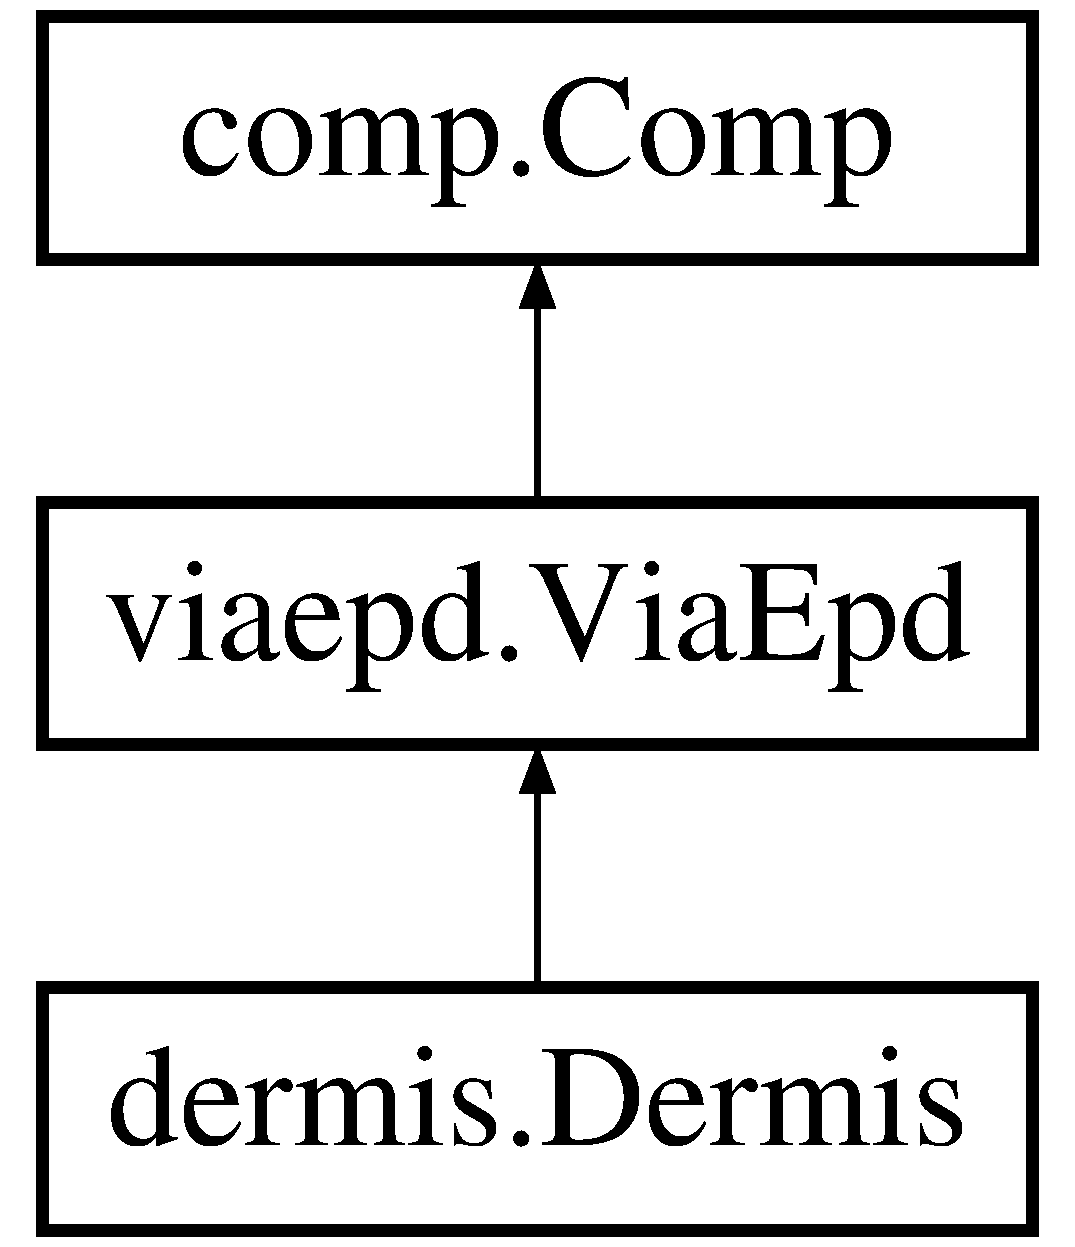
\includegraphics[height=3.000000cm]{classdermis_1_1Dermis}
\end{center}
\end{figure}
\subsection*{Public Member Functions}
\begin{DoxyCompactItemize}
\item 
def {\bfseries \+\_\+\+\_\+init\+\_\+\+\_\+} (self, xlen, ylen, dz\+\_\+dtheta, nx, ny, \hyperlink{classcomp_1_1Comp_ae00e132d485d50acaf13977284fd9051}{coord\+\_\+sys}, bdy\+\_\+cond, \hyperlink{classdermis_1_1Dermis_a274c305d52c6527d75e28bf445a8bb14}{b\+\_\+has\+\_\+blood}=False)\hypertarget{classdermis_1_1Dermis_a16e9e07375f7e75224ed701b13fd5b85}{}\label{classdermis_1_1Dermis_a16e9e07375f7e75224ed701b13fd5b85}

\item 
def {\bfseries get\+\_\+dim} (self)\hypertarget{classdermis_1_1Dermis_a95e926b598eb3ff67d929d51b9845908}{}\label{classdermis_1_1Dermis_a95e926b598eb3ff67d929d51b9845908}

\item 
def {\bfseries get\+Blood\+Conc} (self)\hypertarget{classdermis_1_1Dermis_adc9a75ed6cc17598d5b3cabeed8c1fd1}{}\label{classdermis_1_1Dermis_adc9a75ed6cc17598d5b3cabeed8c1fd1}

\item 
def {\bfseries set\+Blood\+Conc} (self, conc)\hypertarget{classdermis_1_1Dermis_affb1984a8e46447d5b03df8eaaaeb923}{}\label{classdermis_1_1Dermis_affb1984a8e46447d5b03df8eaaaeb923}

\item 
def \hyperlink{classdermis_1_1Dermis_a3444c473db0af2a549683a991a5d1d54}{create\+Dermis\+Blood} (self, bld\+\_\+skin\+\_\+flow, bld\+\_\+fu, par\+\_\+de2blood, bld\+\_\+conc, skin\+\_\+area)
\item 
def \hyperlink{classdermis_1_1Dermis_a05d3cc24f6d0c9b2f3c515e3efde74bc}{create\+Mesh} (self, chem, coord\+\_\+x\+\_\+start, coord\+\_\+y\+\_\+start)
\item 
def \hyperlink{classdermis_1_1Dermis_a25e03ea4853eee1c106c958e9f06c907}{comp\+Par\+Diff} (self, chem)
\item 
def \hyperlink{classdermis_1_1Dermis_a330712627891b74dd3e216910ef913eb}{comp\+O\+D\+Edydt} (self, t, y, args=None)
\begin{DoxyCompactList}\small\item\em (S\+T\+A\+RT OF) Class methods dealing with O\+DE computation \#\#\# \end{DoxyCompactList}\item 
def \hyperlink{classdermis_1_1Dermis_aada0457a4b76448313ff9305df28d9f8}{comp\+O\+D\+Edydt\+\_\+blood} (self, t, y, args=None)
\item 
def \hyperlink{classdermis_1_1Dermis_a75925de5c1db9672a13fa9b409f79376}{save\+Coord} (self, fn\+\_\+x, fn\+\_\+y)\hypertarget{classdermis_1_1Dermis_a75925de5c1db9672a13fa9b409f79376}{}\label{classdermis_1_1Dermis_a75925de5c1db9672a13fa9b409f79376}

\begin{DoxyCompactList}\small\item\em (E\+ND OF) Class methods dealing with O\+DE computation \#\#\# \end{DoxyCompactList}\end{DoxyCompactItemize}
\subsection*{Public Attributes}
\begin{DoxyCompactItemize}
\item 
\hyperlink{classdermis_1_1Dermis_a274c305d52c6527d75e28bf445a8bb14}{b\+\_\+has\+\_\+blood}\hypertarget{classdermis_1_1Dermis_a274c305d52c6527d75e28bf445a8bb14}{}\label{classdermis_1_1Dermis_a274c305d52c6527d75e28bf445a8bb14}

\begin{DoxyCompactList}\small\item\em blood flow ralated varaibles \end{DoxyCompactList}\item 
{\bfseries bld\+\_\+skin\+\_\+flow}\hypertarget{classdermis_1_1Dermis_ad9b92445cf2a99c7adf2d33f59cc368c}{}\label{classdermis_1_1Dermis_ad9b92445cf2a99c7adf2d33f59cc368c}

\item 
{\bfseries bld\+\_\+fu}\hypertarget{classdermis_1_1Dermis_a843f68a56e0fbea2cfeb3fed5810fa60}{}\label{classdermis_1_1Dermis_a843f68a56e0fbea2cfeb3fed5810fa60}

\item 
{\bfseries par\+\_\+de2blood}\hypertarget{classdermis_1_1Dermis_af3cf63fda13e356bc340ca0721761344}{}\label{classdermis_1_1Dermis_af3cf63fda13e356bc340ca0721761344}

\item 
{\bfseries bld\+\_\+conc}\hypertarget{classdermis_1_1Dermis_afdadde0bad3aef09ba5a93b9efc35973}{}\label{classdermis_1_1Dermis_afdadde0bad3aef09ba5a93b9efc35973}

\item 
{\bfseries dermis\+\_\+totalV}\hypertarget{classdermis_1_1Dermis_a488565c2a63a51983eb9104d8d26ffba}{}\label{classdermis_1_1Dermis_a488565c2a63a51983eb9104d8d26ffba}

\item 
{\bfseries mass\+\_\+into\+\_\+dermis}\hypertarget{classdermis_1_1Dermis_a55dd48998cf3bd7743df39e2ecc8b8ea}{}\label{classdermis_1_1Dermis_a55dd48998cf3bd7743df39e2ecc8b8ea}

\item 
{\bfseries mass\+\_\+outof\+\_\+dermis}\hypertarget{classdermis_1_1Dermis_a42c915e7c63d4f7db2531b76dab1702f}{}\label{classdermis_1_1Dermis_a42c915e7c63d4f7db2531b76dab1702f}

\end{DoxyCompactItemize}


\subsection{Detailed Description}
\begin{DoxyVerb}Class definition for Dermis
which is the dermis, currently modelled as a homogenised media,
the same as viable epidermis but with the possibility of
blood flow through
\end{DoxyVerb}
 

Definition at line 15 of file dermis.\+py.



\subsection{Member Function Documentation}
\index{dermis\+::\+Dermis@{dermis\+::\+Dermis}!comp\+O\+D\+Edydt@{comp\+O\+D\+Edydt}}
\index{comp\+O\+D\+Edydt@{comp\+O\+D\+Edydt}!dermis\+::\+Dermis@{dermis\+::\+Dermis}}
\subsubsection[{\texorpdfstring{comp\+O\+D\+Edydt(self, t, y, args=\+None)}{compODEdydt(self, t, y, args=None)}}]{\setlength{\rightskip}{0pt plus 5cm}def dermis.\+Dermis.\+comp\+O\+D\+Edydt (
\begin{DoxyParamCaption}
\item[{}]{self, }
\item[{}]{t, }
\item[{}]{y, }
\item[{}]{args = {\ttfamily None}}
\end{DoxyParamCaption}
)}\hypertarget{classdermis_1_1Dermis_a330712627891b74dd3e216910ef913eb}{}\label{classdermis_1_1Dermis_a330712627891b74dd3e216910ef913eb}


(S\+T\+A\+RT OF) Class methods dealing with O\+DE computation \#\#\# 

\begin{DoxyVerb}The wrapper function for computing the right hand side of ODEs
\end{DoxyVerb}
 

Definition at line 70 of file dermis.\+py.

\index{dermis\+::\+Dermis@{dermis\+::\+Dermis}!comp\+O\+D\+Edydt\+\_\+blood@{comp\+O\+D\+Edydt\+\_\+blood}}
\index{comp\+O\+D\+Edydt\+\_\+blood@{comp\+O\+D\+Edydt\+\_\+blood}!dermis\+::\+Dermis@{dermis\+::\+Dermis}}
\subsubsection[{\texorpdfstring{comp\+O\+D\+Edydt\+\_\+blood(self, t, y, args=\+None)}{compODEdydt_blood(self, t, y, args=None)}}]{\setlength{\rightskip}{0pt plus 5cm}def dermis.\+Dermis.\+comp\+O\+D\+Edydt\+\_\+blood (
\begin{DoxyParamCaption}
\item[{}]{self, }
\item[{}]{t, }
\item[{}]{y, }
\item[{}]{args = {\ttfamily None}}
\end{DoxyParamCaption}
)}\hypertarget{classdermis_1_1Dermis_aada0457a4b76448313ff9305df28d9f8}{}\label{classdermis_1_1Dermis_aada0457a4b76448313ff9305df28d9f8}
\begin{DoxyVerb}Compute the right hand side of ODEs due to blood flow
\end{DoxyVerb}
 

Definition at line 79 of file dermis.\+py.

\index{dermis\+::\+Dermis@{dermis\+::\+Dermis}!comp\+Par\+Diff@{comp\+Par\+Diff}}
\index{comp\+Par\+Diff@{comp\+Par\+Diff}!dermis\+::\+Dermis@{dermis\+::\+Dermis}}
\subsubsection[{\texorpdfstring{comp\+Par\+Diff(self, chem)}{compParDiff(self, chem)}}]{\setlength{\rightskip}{0pt plus 5cm}def dermis.\+Dermis.\+comp\+Par\+Diff (
\begin{DoxyParamCaption}
\item[{}]{self, }
\item[{}]{chem}
\end{DoxyParamCaption}
)}\hypertarget{classdermis_1_1Dermis_a25e03ea4853eee1c106c958e9f06c907}{}\label{classdermis_1_1Dermis_a25e03ea4853eee1c106c958e9f06c907}
\begin{DoxyVerb}Compute the partition coefficient with respect to water
and the diffusion coefficient
\end{DoxyVerb}
 

Definition at line 61 of file dermis.\+py.

\index{dermis\+::\+Dermis@{dermis\+::\+Dermis}!create\+Dermis\+Blood@{create\+Dermis\+Blood}}
\index{create\+Dermis\+Blood@{create\+Dermis\+Blood}!dermis\+::\+Dermis@{dermis\+::\+Dermis}}
\subsubsection[{\texorpdfstring{create\+Dermis\+Blood(self, bld\+\_\+skin\+\_\+flow, bld\+\_\+fu, par\+\_\+de2blood, bld\+\_\+conc, skin\+\_\+area)}{createDermisBlood(self, bld_skin_flow, bld_fu, par_de2blood, bld_conc, skin_area)}}]{\setlength{\rightskip}{0pt plus 5cm}def dermis.\+Dermis.\+create\+Dermis\+Blood (
\begin{DoxyParamCaption}
\item[{}]{self, }
\item[{}]{bld\+\_\+skin\+\_\+flow, }
\item[{}]{bld\+\_\+fu, }
\item[{}]{par\+\_\+de2blood, }
\item[{}]{bld\+\_\+conc, }
\item[{}]{skin\+\_\+area}
\end{DoxyParamCaption}
)}\hypertarget{classdermis_1_1Dermis_a3444c473db0af2a549683a991a5d1d54}{}\label{classdermis_1_1Dermis_a3444c473db0af2a549683a991a5d1d54}
\begin{DoxyVerb}Create variables relating to blood flow
\end{DoxyVerb}
 

Definition at line 42 of file dermis.\+py.

\index{dermis\+::\+Dermis@{dermis\+::\+Dermis}!create\+Mesh@{create\+Mesh}}
\index{create\+Mesh@{create\+Mesh}!dermis\+::\+Dermis@{dermis\+::\+Dermis}}
\subsubsection[{\texorpdfstring{create\+Mesh(self, chem, coord\+\_\+x\+\_\+start, coord\+\_\+y\+\_\+start)}{createMesh(self, chem, coord_x_start, coord_y_start)}}]{\setlength{\rightskip}{0pt plus 5cm}def dermis.\+Dermis.\+create\+Mesh (
\begin{DoxyParamCaption}
\item[{}]{self, }
\item[{}]{chem, }
\item[{}]{coord\+\_\+x\+\_\+start, }
\item[{}]{coord\+\_\+y\+\_\+start}
\end{DoxyParamCaption}
)}\hypertarget{classdermis_1_1Dermis_a05d3cc24f6d0c9b2f3c515e3efde74bc}{}\label{classdermis_1_1Dermis_a05d3cc24f6d0c9b2f3c515e3efde74bc}
\begin{DoxyVerb}Create mesh for this compartment
Args:
coord_x_start, coord_y_start: starting coordinates
\end{DoxyVerb}
 

Definition at line 52 of file dermis.\+py.



The documentation for this class was generated from the following file\+:\begin{DoxyCompactItemize}
\item 
dermis.\+py\end{DoxyCompactItemize}

\hypertarget{classmesh_1_1Mesh}{}\section{mesh.\+Mesh Class Reference}
\label{classmesh_1_1Mesh}\index{mesh.\+Mesh@{mesh.\+Mesh}}
\subsection*{Public Member Functions}
\begin{DoxyCompactItemize}
\item 
def \hyperlink{classmesh_1_1Mesh_a016f17ce91fada2b8c3d3f5b16cce9b4}{\+\_\+\+\_\+init\+\_\+\+\_\+} (self, name=None, chem, conc, Kw, D, x\+\_\+coord, y\+\_\+coord, dx, dy, dz)
\item 
def {\bfseries get\+\_\+dx} (self)\hypertarget{classmesh_1_1Mesh_aac1703ed48d76086e368185b22379f7c}{}\label{classmesh_1_1Mesh_aac1703ed48d76086e368185b22379f7c}

\item 
def {\bfseries set\+\_\+dx} (self, dx)\hypertarget{classmesh_1_1Mesh_ad40facc36923c9b0fcc0d6363ee6107b}{}\label{classmesh_1_1Mesh_ad40facc36923c9b0fcc0d6363ee6107b}

\item 
def {\bfseries get\+\_\+dy} (self)\hypertarget{classmesh_1_1Mesh_aef4bece754687fe2a3ae90e07829913d}{}\label{classmesh_1_1Mesh_aef4bece754687fe2a3ae90e07829913d}

\item 
def {\bfseries set\+\_\+dy} (self, dy)\hypertarget{classmesh_1_1Mesh_a7f1c6bb5694f587777f426da7c316aa3}{}\label{classmesh_1_1Mesh_a7f1c6bb5694f587777f426da7c316aa3}

\item 
def {\bfseries get\+\_\+x\+\_\+coord} (self)\hypertarget{classmesh_1_1Mesh_af4cefc4542a761b56edd215265b8d367}{}\label{classmesh_1_1Mesh_af4cefc4542a761b56edd215265b8d367}

\item 
def {\bfseries set\+\_\+x\+\_\+coord} (self, x\+\_\+coord)\hypertarget{classmesh_1_1Mesh_ac7be9a536451cb577ebf0ce4debc43c1}{}\label{classmesh_1_1Mesh_ac7be9a536451cb577ebf0ce4debc43c1}

\item 
def {\bfseries get\+Conc} (self)\hypertarget{classmesh_1_1Mesh_a0a358fc09db4af0d46d696bb796bca66}{}\label{classmesh_1_1Mesh_a0a358fc09db4af0d46d696bb796bca66}

\item 
def {\bfseries set\+Conc} (self, conc)\hypertarget{classmesh_1_1Mesh_ad5802c6f926a2fe0d7b885c9c687a5da}{}\label{classmesh_1_1Mesh_ad5802c6f926a2fe0d7b885c9c687a5da}

\item 
def {\bfseries get\+\_\+no\+\_\+species} (self)\hypertarget{classmesh_1_1Mesh_adf05f4be209e9171d147e66763b3f206}{}\label{classmesh_1_1Mesh_adf05f4be209e9171d147e66763b3f206}

\item 
def {\bfseries set\+\_\+no\+\_\+species} (self, n)\hypertarget{classmesh_1_1Mesh_a65d4a784781429cff8e3d20d3741c63f}{}\label{classmesh_1_1Mesh_a65d4a784781429cff8e3d20d3741c63f}

\item 
def \hyperlink{classmesh_1_1Mesh_a5d79b848ed97ec98bd97f92ed7989c66}{comp\+Inter\+Area} (self, direction)
\begin{DoxyCompactList}\small\item\em (S\+T\+A\+RT OF) Class methods dealing with geometries \#\#\# \end{DoxyCompactList}\item 
def {\bfseries comp\+Volume} (self)\hypertarget{classmesh_1_1Mesh_ab045aecb3cc2168b185060f7b59f3b6d}{}\label{classmesh_1_1Mesh_ab045aecb3cc2168b185060f7b59f3b6d}

\end{DoxyCompactItemize}
\subsection*{Public Attributes}
\begin{DoxyCompactItemize}
\item 
{\bfseries name}\hypertarget{classmesh_1_1Mesh_a1f98e9af552cbb4fb998e0ac377b7fe9}{}\label{classmesh_1_1Mesh_a1f98e9af552cbb4fb998e0ac377b7fe9}

\item 
{\bfseries chem}\hypertarget{classmesh_1_1Mesh_a27e17a523b77a2196a520da01e503572}{}\label{classmesh_1_1Mesh_a27e17a523b77a2196a520da01e503572}

\item 
{\bfseries n\+Species}\hypertarget{classmesh_1_1Mesh_ab1fa480cfc187a684e22ec48f667f95e}{}\label{classmesh_1_1Mesh_ab1fa480cfc187a684e22ec48f667f95e}

\item 
{\bfseries conc}\hypertarget{classmesh_1_1Mesh_aa96d78fc94879b016e4db2fe931ec06a}{}\label{classmesh_1_1Mesh_aa96d78fc94879b016e4db2fe931ec06a}

\item 
{\bfseries Kw}\hypertarget{classmesh_1_1Mesh_ad0d830cae9f3f27065687c42bf59b2d5}{}\label{classmesh_1_1Mesh_ad0d830cae9f3f27065687c42bf59b2d5}

\item 
{\bfseries D}\hypertarget{classmesh_1_1Mesh_a60ec58712923b46771ab2d445b82f3e1}{}\label{classmesh_1_1Mesh_a60ec58712923b46771ab2d445b82f3e1}

\item 
{\bfseries x\+\_\+coord}\hypertarget{classmesh_1_1Mesh_ab25a51d16acccd8faf52ce1561131eac}{}\label{classmesh_1_1Mesh_ab25a51d16acccd8faf52ce1561131eac}

\item 
{\bfseries y\+\_\+coord}\hypertarget{classmesh_1_1Mesh_af375fec3a82063091d646d269acedb11}{}\label{classmesh_1_1Mesh_af375fec3a82063091d646d269acedb11}

\item 
{\bfseries dx}\hypertarget{classmesh_1_1Mesh_aa7eaed4128e4da7110be30a0e6735622}{}\label{classmesh_1_1Mesh_aa7eaed4128e4da7110be30a0e6735622}

\item 
{\bfseries dy}\hypertarget{classmesh_1_1Mesh_af3e53234aa182066213c20b1153bc79e}{}\label{classmesh_1_1Mesh_af3e53234aa182066213c20b1153bc79e}

\item 
{\bfseries dz}\hypertarget{classmesh_1_1Mesh_a6d9d205c0c3dbec64f3e047d0a03650b}{}\label{classmesh_1_1Mesh_a6d9d205c0c3dbec64f3e047d0a03650b}

\item 
{\bfseries coord\+\_\+sys}\hypertarget{classmesh_1_1Mesh_a36f45477e36cc4b8b29052a1006a1e10}{}\label{classmesh_1_1Mesh_a36f45477e36cc4b8b29052a1006a1e10}

\end{DoxyCompactItemize}


\subsection{Detailed Description}
\begin{DoxyVerb}Class definition for Mesh.
\end{DoxyVerb}
 

Definition at line 11 of file mesh.\+py.



\subsection{Constructor \& Destructor Documentation}
\index{mesh\+::\+Mesh@{mesh\+::\+Mesh}!\+\_\+\+\_\+init\+\_\+\+\_\+@{\+\_\+\+\_\+init\+\_\+\+\_\+}}
\index{\+\_\+\+\_\+init\+\_\+\+\_\+@{\+\_\+\+\_\+init\+\_\+\+\_\+}!mesh\+::\+Mesh@{mesh\+::\+Mesh}}
\subsubsection[{\texorpdfstring{\+\_\+\+\_\+init\+\_\+\+\_\+(self, name=\+None, chem, conc, Kw, D, x\+\_\+coord, y\+\_\+coord, dx, dy, dz)}{__init__(self, name=None, chem, conc, Kw, D, x_coord, y_coord, dx, dy, dz)}}]{\setlength{\rightskip}{0pt plus 5cm}def mesh.\+Mesh.\+\_\+\+\_\+init\+\_\+\+\_\+ (
\begin{DoxyParamCaption}
\item[{}]{self, }
\item[{}]{name = {\ttfamily None}, }
\item[{}]{chem, }
\item[{}]{conc, }
\item[{}]{Kw, }
\item[{}]{D, }
\item[{}]{x\+\_\+coord, }
\item[{}]{y\+\_\+coord, }
\item[{}]{dx, }
\item[{}]{dy, }
\item[{}]{dz}
\end{DoxyParamCaption}
)}\hypertarget{classmesh_1_1Mesh_a016f17ce91fada2b8c3d3f5b16cce9b4}{}\label{classmesh_1_1Mesh_a016f17ce91fada2b8c3d3f5b16cce9b4}
\begin{DoxyVerb}Args:
    Kw, D - partition and diffusion coefficients in this mesh
\end{DoxyVerb}
 

Definition at line 18 of file mesh.\+py.



\subsection{Member Function Documentation}
\index{mesh\+::\+Mesh@{mesh\+::\+Mesh}!comp\+Inter\+Area@{comp\+Inter\+Area}}
\index{comp\+Inter\+Area@{comp\+Inter\+Area}!mesh\+::\+Mesh@{mesh\+::\+Mesh}}
\subsubsection[{\texorpdfstring{comp\+Inter\+Area(self, direction)}{compInterArea(self, direction)}}]{\setlength{\rightskip}{0pt plus 5cm}def mesh.\+Mesh.\+comp\+Inter\+Area (
\begin{DoxyParamCaption}
\item[{}]{self, }
\item[{}]{direction}
\end{DoxyParamCaption}
)}\hypertarget{classmesh_1_1Mesh_a5d79b848ed97ec98bd97f92ed7989c66}{}\label{classmesh_1_1Mesh_a5d79b848ed97ec98bd97f92ed7989c66}


(S\+T\+A\+RT OF) Class methods dealing with geometries \#\#\# 

\begin{DoxyVerb}Calculate the interfacial area between self and a neighbouring mesh
direction: [0] = up; [1] = left; [2] = right; [3] = down
\end{DoxyVerb}
 

Definition at line 61 of file mesh.\+py.



The documentation for this class was generated from the following file\+:\begin{DoxyCompactItemize}
\item 
mesh.\+py\end{DoxyCompactItemize}

\hypertarget{classmesh_1_1MeshSink}{}\section{mesh.\+Mesh\+Sink Class Reference}
\label{classmesh_1_1MeshSink}\index{mesh.\+Mesh\+Sink@{mesh.\+Mesh\+Sink}}
Inheritance diagram for mesh.\+Mesh\+Sink\+:\begin{figure}[H]
\begin{center}
\leavevmode
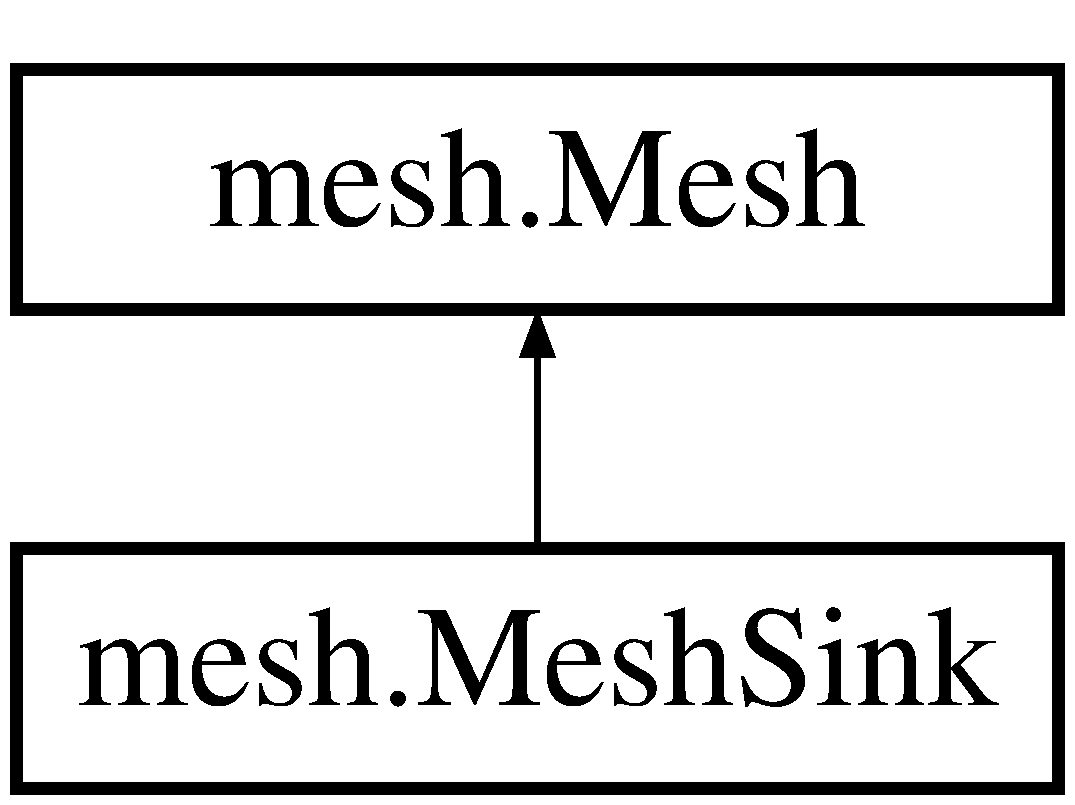
\includegraphics[height=2.000000cm]{classmesh_1_1MeshSink}
\end{center}
\end{figure}
\subsection*{Public Member Functions}
\begin{DoxyCompactItemize}
\item 
def {\bfseries \+\_\+\+\_\+init\+\_\+\+\_\+} (self)\hypertarget{classmesh_1_1MeshSink_ac5f16f1f0460e35ac224125975761f18}{}\label{classmesh_1_1MeshSink_ac5f16f1f0460e35ac224125975761f18}

\end{DoxyCompactItemize}
\subsection*{Additional Inherited Members}


\subsection{Detailed Description}
\begin{DoxyVerb}Derive a Sink class from Mesh
\end{DoxyVerb}
 

Definition at line 152 of file mesh.\+py.



The documentation for this class was generated from the following file\+:\begin{DoxyCompactItemize}
\item 
mesh.\+py\end{DoxyCompactItemize}

\hypertarget{classpoint_1_1Point}{}\section{point.\+Point Class Reference}
\label{classpoint_1_1Point}\index{point.\+Point@{point.\+Point}}
\subsection*{Public Member Functions}
\begin{DoxyCompactItemize}
\item 
def {\bfseries \+\_\+\+\_\+init\+\_\+\+\_\+} (self, x\+\_\+coord, y\+\_\+coord, dx, dy, x\+\_\+type, y\+\_\+type)\hypertarget{classpoint_1_1Point_ad828850bdd90bf5a031f787e15a67f22}{}\label{classpoint_1_1Point_ad828850bdd90bf5a031f787e15a67f22}

\item 
def \hyperlink{classpoint_1_1Point_a5c98be41b46b735c986f0c0bd0f296e2}{set\+Point} (self, x\+\_\+coord, y\+\_\+coord, dx, dy, x\+\_\+type, y\+\_\+type)
\item 
def \hyperlink{classpoint_1_1Point_a24b1b672d23a397aad796aaa9c1e5f61}{cpy\+Point} (self, source\+\_\+point)
\end{DoxyCompactItemize}
\subsection*{Public Attributes}
\begin{DoxyCompactItemize}
\item 
{\bfseries x\+\_\+coord}\hypertarget{classpoint_1_1Point_ac8519ea666c81f170f0be398c40aad1f}{}\label{classpoint_1_1Point_ac8519ea666c81f170f0be398c40aad1f}

\item 
{\bfseries y\+\_\+coord}\hypertarget{classpoint_1_1Point_a9b956d382d3a6db5a39aa5895f9a5ab8}{}\label{classpoint_1_1Point_a9b956d382d3a6db5a39aa5895f9a5ab8}

\item 
{\bfseries dx}\hypertarget{classpoint_1_1Point_ae686cba0fd4073a678fbe82848477a2d}{}\label{classpoint_1_1Point_ae686cba0fd4073a678fbe82848477a2d}

\item 
{\bfseries dy}\hypertarget{classpoint_1_1Point_a828d51f1faabddb60a6eb4a31a024de6}{}\label{classpoint_1_1Point_a828d51f1faabddb60a6eb4a31a024de6}

\item 
{\bfseries x\+\_\+type}\hypertarget{classpoint_1_1Point_af62100393bbf1847f68d0cb76c3f9700}{}\label{classpoint_1_1Point_af62100393bbf1847f68d0cb76c3f9700}

\item 
{\bfseries y\+\_\+type}\hypertarget{classpoint_1_1Point_a37d1b32204ade133d4da0c7826cfe9f9}{}\label{classpoint_1_1Point_a37d1b32204ade133d4da0c7826cfe9f9}

\end{DoxyCompactItemize}


\subsection{Detailed Description}
\begin{DoxyVerb}Class definition for Point
which is a specific point in space
\end{DoxyVerb}
 

Definition at line 9 of file point.\+py.



\subsection{Member Function Documentation}
\index{point\+::\+Point@{point\+::\+Point}!cpy\+Point@{cpy\+Point}}
\index{cpy\+Point@{cpy\+Point}!point\+::\+Point@{point\+::\+Point}}
\subsubsection[{\texorpdfstring{cpy\+Point(self, source\+\_\+point)}{cpyPoint(self, source_point)}}]{\setlength{\rightskip}{0pt plus 5cm}def point.\+Point.\+cpy\+Point (
\begin{DoxyParamCaption}
\item[{}]{self, }
\item[{}]{source\+\_\+point}
\end{DoxyParamCaption}
)}\hypertarget{classpoint_1_1Point_a24b1b672d23a397aad796aaa9c1e5f61}{}\label{classpoint_1_1Point_a24b1b672d23a397aad796aaa9c1e5f61}
\begin{DoxyVerb}\end{DoxyVerb}
 

Definition at line 27 of file point.\+py.

\index{point\+::\+Point@{point\+::\+Point}!set\+Point@{set\+Point}}
\index{set\+Point@{set\+Point}!point\+::\+Point@{point\+::\+Point}}
\subsubsection[{\texorpdfstring{set\+Point(self, x\+\_\+coord, y\+\_\+coord, dx, dy, x\+\_\+type, y\+\_\+type)}{setPoint(self, x_coord, y_coord, dx, dy, x_type, y_type)}}]{\setlength{\rightskip}{0pt plus 5cm}def point.\+Point.\+set\+Point (
\begin{DoxyParamCaption}
\item[{}]{self, }
\item[{}]{x\+\_\+coord, }
\item[{}]{y\+\_\+coord, }
\item[{}]{dx, }
\item[{}]{dy, }
\item[{}]{x\+\_\+type, }
\item[{}]{y\+\_\+type}
\end{DoxyParamCaption}
)}\hypertarget{classpoint_1_1Point_a5c98be41b46b735c986f0c0bd0f296e2}{}\label{classpoint_1_1Point_a5c98be41b46b735c986f0c0bd0f296e2}
\begin{DoxyVerb}\end{DoxyVerb}
 

Definition at line 17 of file point.\+py.



The documentation for this class was generated from the following file\+:\begin{DoxyCompactItemize}
\item 
point.\+py\end{DoxyCompactItemize}

\hypertarget{classskin_1_1Skin}{}\section{skin.\+Skin Class Reference}
\label{classskin_1_1Skin}\index{skin.\+Skin@{skin.\+Skin}}
\subsection*{Public Member Functions}
\begin{DoxyCompactItemize}
\item 
def {\bfseries \+\_\+\+\_\+init\+\_\+\+\_\+} (self, coord\+\_\+sys=None, dz\+\_\+dtheta=None, bdy\+\_\+cond=None)\hypertarget{classskin_1_1Skin_ae8c14fb876f2b90c955f4914df5ecde4}{}\label{classskin_1_1Skin_ae8c14fb876f2b90c955f4914df5ecde4}

\item 
def \hyperlink{classskin_1_1Skin_ae9dae685416ddd7e3f345a3ff6449998}{comp\+O\+D\+Edydt\+\_\+diffu} (self, t, y, args=None)
\begin{DoxyCompactList}\small\item\em (S\+T\+A\+RT OF) Class methods dealing with O\+DE computation \#\#\# \end{DoxyCompactList}\item 
def \hyperlink{classskin_1_1Skin_aefaa68f4f0d659f05aa2babeafbe1995}{solve\+MoL} (self, t\+\_\+start, t\+\_\+end)
\item 
def \hyperlink{classskin_1_1Skin_a411a39ab1c8faf9faa3fb6c8bea777f9}{get\+Bdy\+Right} (self, comp\+This, y, idx\+\_\+up2now, c\+Idx\+\_\+i, c\+Idx\+\_\+j)
\begin{DoxyCompactList}\small\item\em (E\+ND OF) Class methods dealing with O\+DE computation \#\#\# \end{DoxyCompactList}\item 
def \hyperlink{classskin_1_1Skin_a477a800e6beba99197c2744ebcdc5426}{get\+Bdy\+Down} (self, comp\+This, y, idx\+\_\+up2now, c\+Idx\+\_\+i, c\+Idx\+\_\+j)
\end{DoxyCompactItemize}
\subsection*{Public Attributes}
\begin{DoxyCompactItemize}
\item 
{\bfseries comps}\hypertarget{classskin_1_1Skin_ac0a2c5b23d7f0f6e69edb6f666c6a8fc}{}\label{classskin_1_1Skin_ac0a2c5b23d7f0f6e69edb6f666c6a8fc}

\end{DoxyCompactItemize}


\subsection{Detailed Description}
\begin{DoxyVerb}Class definition for Skin
which can contain a number of compartments
\end{DoxyVerb}
 

Definition at line 13 of file skin.\+py.



\subsection{Member Function Documentation}
\index{skin\+::\+Skin@{skin\+::\+Skin}!comp\+O\+D\+Edydt\+\_\+diffu@{comp\+O\+D\+Edydt\+\_\+diffu}}
\index{comp\+O\+D\+Edydt\+\_\+diffu@{comp\+O\+D\+Edydt\+\_\+diffu}!skin\+::\+Skin@{skin\+::\+Skin}}
\subsubsection[{\texorpdfstring{comp\+O\+D\+Edydt\+\_\+diffu(self, t, y, args=\+None)}{compODEdydt_diffu(self, t, y, args=None)}}]{\setlength{\rightskip}{0pt plus 5cm}def skin.\+Skin.\+comp\+O\+D\+Edydt\+\_\+diffu (
\begin{DoxyParamCaption}
\item[{}]{self, }
\item[{}]{t, }
\item[{}]{y, }
\item[{}]{args = {\ttfamily None}}
\end{DoxyParamCaption}
)}\hypertarget{classskin_1_1Skin_ae9dae685416ddd7e3f345a3ff6449998}{}\label{classskin_1_1Skin_ae9dae685416ddd7e3f345a3ff6449998}


(S\+T\+A\+RT OF) Class methods dealing with O\+DE computation \#\#\# 

\begin{DoxyVerb}Compute the right-hand side of the ODEs, i.e. dydt, due to diffusion
\end{DoxyVerb}
 

Definition at line 26 of file skin.\+py.

\index{skin\+::\+Skin@{skin\+::\+Skin}!get\+Bdy\+Down@{get\+Bdy\+Down}}
\index{get\+Bdy\+Down@{get\+Bdy\+Down}!skin\+::\+Skin@{skin\+::\+Skin}}
\subsubsection[{\texorpdfstring{get\+Bdy\+Down(self, comp\+This, y, idx\+\_\+up2now, c\+Idx\+\_\+i, c\+Idx\+\_\+j)}{getBdyDown(self, compThis, y, idx_up2now, cIdx_i, cIdx_j)}}]{\setlength{\rightskip}{0pt plus 5cm}def skin.\+Skin.\+get\+Bdy\+Down (
\begin{DoxyParamCaption}
\item[{}]{self, }
\item[{}]{comp\+This, }
\item[{}]{y, }
\item[{}]{idx\+\_\+up2now, }
\item[{}]{c\+Idx\+\_\+i, }
\item[{}]{c\+Idx\+\_\+j}
\end{DoxyParamCaption}
)}\hypertarget{classskin_1_1Skin_a477a800e6beba99197c2744ebcdc5426}{}\label{classskin_1_1Skin_a477a800e6beba99197c2744ebcdc5426}
\begin{DoxyVerb}Get the boundary to the down of this compartment
using values in y[]
\end{DoxyVerb}
 

Definition at line 139 of file skin.\+py.

\index{skin\+::\+Skin@{skin\+::\+Skin}!get\+Bdy\+Right@{get\+Bdy\+Right}}
\index{get\+Bdy\+Right@{get\+Bdy\+Right}!skin\+::\+Skin@{skin\+::\+Skin}}
\subsubsection[{\texorpdfstring{get\+Bdy\+Right(self, comp\+This, y, idx\+\_\+up2now, c\+Idx\+\_\+i, c\+Idx\+\_\+j)}{getBdyRight(self, compThis, y, idx_up2now, cIdx_i, cIdx_j)}}]{\setlength{\rightskip}{0pt plus 5cm}def skin.\+Skin.\+get\+Bdy\+Right (
\begin{DoxyParamCaption}
\item[{}]{self, }
\item[{}]{comp\+This, }
\item[{}]{y, }
\item[{}]{idx\+\_\+up2now, }
\item[{}]{c\+Idx\+\_\+i, }
\item[{}]{c\+Idx\+\_\+j}
\end{DoxyParamCaption}
)}\hypertarget{classskin_1_1Skin_a411a39ab1c8faf9faa3fb6c8bea777f9}{}\label{classskin_1_1Skin_a411a39ab1c8faf9faa3fb6c8bea777f9}


(E\+ND OF) Class methods dealing with O\+DE computation \#\#\# 

(S\+T\+A\+RT OF) Class methods dealing with boundaries \#\#\# \begin{DoxyVerb}Get the boundary to the right of this compartment
using values in y[]
\end{DoxyVerb}
 

Definition at line 118 of file skin.\+py.

\index{skin\+::\+Skin@{skin\+::\+Skin}!solve\+MoL@{solve\+MoL}}
\index{solve\+MoL@{solve\+MoL}!skin\+::\+Skin@{skin\+::\+Skin}}
\subsubsection[{\texorpdfstring{solve\+Mo\+L(self, t\+\_\+start, t\+\_\+end)}{solveMoL(self, t_start, t_end)}}]{\setlength{\rightskip}{0pt plus 5cm}def skin.\+Skin.\+solve\+MoL (
\begin{DoxyParamCaption}
\item[{}]{self, }
\item[{}]{t\+\_\+start, }
\item[{}]{t\+\_\+end}
\end{DoxyParamCaption}
)}\hypertarget{classskin_1_1Skin_aefaa68f4f0d659f05aa2babeafbe1995}{}\label{classskin_1_1Skin_aefaa68f4f0d659f05aa2babeafbe1995}
\begin{DoxyVerb}Solving PDE using method of lines (MoL)
\end{DoxyVerb}
 

Definition at line 75 of file skin.\+py.



The documentation for this class was generated from the following file\+:\begin{DoxyCompactItemize}
\item 
skin.\+py\end{DoxyCompactItemize}

\hypertarget{classskin__setup_1_1Skin__Setup}{}\section{skin\+\_\+setup.\+Skin\+\_\+\+Setup Class Reference}
\label{classskin__setup_1_1Skin__Setup}\index{skin\+\_\+setup.\+Skin\+\_\+\+Setup@{skin\+\_\+setup.\+Skin\+\_\+\+Setup}}
Inheritance diagram for skin\+\_\+setup.\+Skin\+\_\+\+Setup\+:\begin{figure}[H]
\begin{center}
\leavevmode
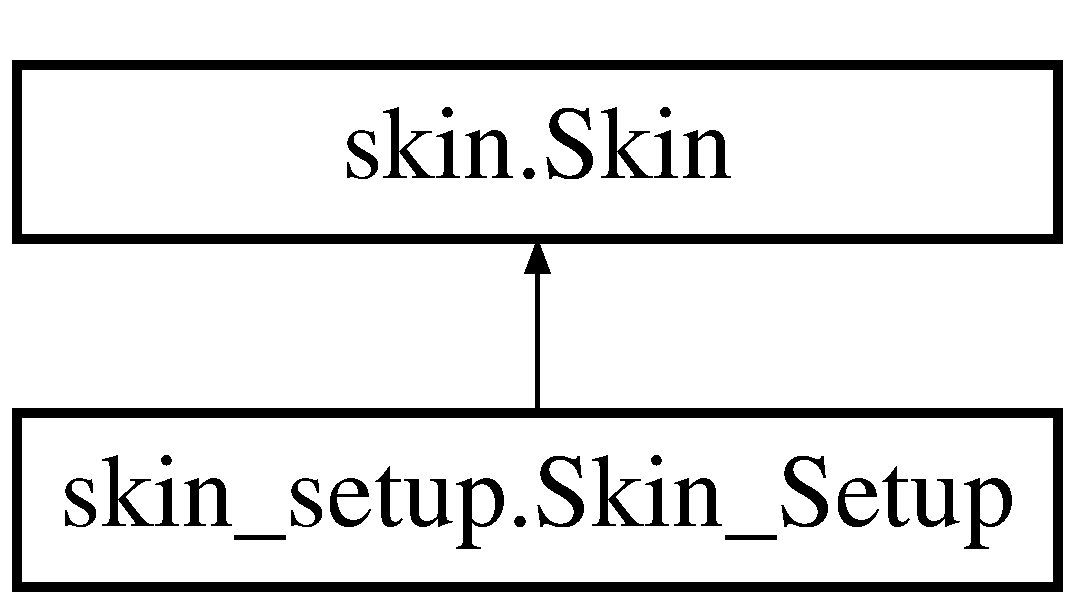
\includegraphics[height=2.000000cm]{classskin__setup_1_1Skin__Setup}
\end{center}
\end{figure}
\subsection*{Public Member Functions}
\begin{DoxyCompactItemize}
\item 
def {\bfseries \+\_\+\+\_\+init\+\_\+\+\_\+} (self, chem, conf)\hypertarget{classskin__setup_1_1Skin__Setup_a2611544358a7178751abaf0d2d98c931}{}\label{classskin__setup_1_1Skin__Setup_a2611544358a7178751abaf0d2d98c931}

\item 
def \hyperlink{classskin__setup_1_1Skin__Setup_aeb7289f58a76638e31e24e71ae186309}{create\+Comps} (self, chem, conf)
\item 
def \hyperlink{classskin__setup_1_1Skin__Setup_a080759893083f543703f6b4f17ae6260}{create\+SC} (self, chem, coord\+\_\+x\+\_\+start, coord\+\_\+y\+\_\+start, n\+\_\+layer\+\_\+x, n\+\_\+layer\+\_\+y, offset\+\_\+y, bdy\+Cond)
\begin{DoxyCompactList}\small\item\em (S\+T\+A\+RT OF) Create individual compartments \#\#\# \end{DoxyCompactList}\item 
def \hyperlink{classskin__setup_1_1Skin__Setup_a0271f9e73005e8c52c3b397edb534881}{create\+VE} (self, chem, coord\+\_\+x\+\_\+start, coord\+\_\+y\+\_\+start, xlen, ylen, n\+\_\+grids\+\_\+x, n\+\_\+grids\+\_\+y, bdy\+Cond)
\item 
def \hyperlink{classskin__setup_1_1Skin__Setup_a147ae38354fa1c30b2cb6b911a785e19}{create\+DE} (self, chem, coord\+\_\+x\+\_\+start, coord\+\_\+y\+\_\+start, xlen, ylen, n\+\_\+grids\+\_\+x, n\+\_\+grids\+\_\+y, bdy\+Cond)
\end{DoxyCompactItemize}
\subsection*{Public Attributes}
\begin{DoxyCompactItemize}
\item 
{\bfseries comp\+\_\+structure}\hypertarget{classskin__setup_1_1Skin__Setup_a8b09dae390dec5b69a401098955f3b1b}{}\label{classskin__setup_1_1Skin__Setup_a8b09dae390dec5b69a401098955f3b1b}

\item 
{\bfseries b\+\_\+has\+\_\+blood}\hypertarget{classskin__setup_1_1Skin__Setup_aead0a66ccc670a27de3f87fab70ab5b9}{}\label{classskin__setup_1_1Skin__Setup_aead0a66ccc670a27de3f87fab70ab5b9}

\end{DoxyCompactItemize}


\subsection{Detailed Description}
\begin{DoxyVerb}Class definition for Skin_Setup
which intends to set up the compartments in simulation as instructed by user
\end{DoxyVerb}
 

Definition at line 18 of file skin\+\_\+setup.\+py.



\subsection{Member Function Documentation}
\index{skin\+\_\+setup\+::\+Skin\+\_\+\+Setup@{skin\+\_\+setup\+::\+Skin\+\_\+\+Setup}!create\+Comps@{create\+Comps}}
\index{create\+Comps@{create\+Comps}!skin\+\_\+setup\+::\+Skin\+\_\+\+Setup@{skin\+\_\+setup\+::\+Skin\+\_\+\+Setup}}
\subsubsection[{\texorpdfstring{create\+Comps(self, chem, conf)}{createComps(self, chem, conf)}}]{\setlength{\rightskip}{0pt plus 5cm}def skin\+\_\+setup.\+Skin\+\_\+\+Setup.\+create\+Comps (
\begin{DoxyParamCaption}
\item[{}]{self, }
\item[{}]{chem, }
\item[{}]{conf}
\end{DoxyParamCaption}
)}\hypertarget{classskin__setup_1_1Skin__Setup_aeb7289f58a76638e31e24e71ae186309}{}\label{classskin__setup_1_1Skin__Setup_aeb7289f58a76638e31e24e71ae186309}
\begin{DoxyVerb}Create compartments
Letter code:
    V: vehicle            S: stratum cornuem
    E: viable epidermis   D: dermis
    B: blood              H: Hair
\end{DoxyVerb}
 

Definition at line 38 of file skin\+\_\+setup.\+py.

\index{skin\+\_\+setup\+::\+Skin\+\_\+\+Setup@{skin\+\_\+setup\+::\+Skin\+\_\+\+Setup}!create\+DE@{create\+DE}}
\index{create\+DE@{create\+DE}!skin\+\_\+setup\+::\+Skin\+\_\+\+Setup@{skin\+\_\+setup\+::\+Skin\+\_\+\+Setup}}
\subsubsection[{\texorpdfstring{create\+D\+E(self, chem, coord\+\_\+x\+\_\+start, coord\+\_\+y\+\_\+start, xlen, ylen, n\+\_\+grids\+\_\+x, n\+\_\+grids\+\_\+y, bdy\+Cond)}{createDE(self, chem, coord_x_start, coord_y_start, xlen, ylen, n_grids_x, n_grids_y, bdyCond)}}]{\setlength{\rightskip}{0pt plus 5cm}def skin\+\_\+setup.\+Skin\+\_\+\+Setup.\+create\+DE (
\begin{DoxyParamCaption}
\item[{}]{self, }
\item[{}]{chem, }
\item[{}]{coord\+\_\+x\+\_\+start, }
\item[{}]{coord\+\_\+y\+\_\+start, }
\item[{}]{xlen, }
\item[{}]{ylen, }
\item[{}]{n\+\_\+grids\+\_\+x, }
\item[{}]{n\+\_\+grids\+\_\+y, }
\item[{}]{bdy\+Cond}
\end{DoxyParamCaption}
)}\hypertarget{classskin__setup_1_1Skin__Setup_a147ae38354fa1c30b2cb6b911a785e19}{}\label{classskin__setup_1_1Skin__Setup_a147ae38354fa1c30b2cb6b911a785e19}
\begin{DoxyVerb}Create dermis \end{DoxyVerb}
 

Definition at line 143 of file skin\+\_\+setup.\+py.

\index{skin\+\_\+setup\+::\+Skin\+\_\+\+Setup@{skin\+\_\+setup\+::\+Skin\+\_\+\+Setup}!create\+SC@{create\+SC}}
\index{create\+SC@{create\+SC}!skin\+\_\+setup\+::\+Skin\+\_\+\+Setup@{skin\+\_\+setup\+::\+Skin\+\_\+\+Setup}}
\subsubsection[{\texorpdfstring{create\+S\+C(self, chem, coord\+\_\+x\+\_\+start, coord\+\_\+y\+\_\+start, n\+\_\+layer\+\_\+x, n\+\_\+layer\+\_\+y, offset\+\_\+y, bdy\+Cond)}{createSC(self, chem, coord_x_start, coord_y_start, n_layer_x, n_layer_y, offset_y, bdyCond)}}]{\setlength{\rightskip}{0pt plus 5cm}def skin\+\_\+setup.\+Skin\+\_\+\+Setup.\+create\+SC (
\begin{DoxyParamCaption}
\item[{}]{self, }
\item[{}]{chem, }
\item[{}]{coord\+\_\+x\+\_\+start, }
\item[{}]{coord\+\_\+y\+\_\+start, }
\item[{}]{n\+\_\+layer\+\_\+x, }
\item[{}]{n\+\_\+layer\+\_\+y, }
\item[{}]{offset\+\_\+y, }
\item[{}]{bdy\+Cond}
\end{DoxyParamCaption}
)}\hypertarget{classskin__setup_1_1Skin__Setup_a080759893083f543703f6b4f17ae6260}{}\label{classskin__setup_1_1Skin__Setup_a080759893083f543703f6b4f17ae6260}


(S\+T\+A\+RT OF) Create individual compartments \#\#\# 

\begin{DoxyVerb}Create stratum corneum \end{DoxyVerb}
 

Definition at line 126 of file skin\+\_\+setup.\+py.

\index{skin\+\_\+setup\+::\+Skin\+\_\+\+Setup@{skin\+\_\+setup\+::\+Skin\+\_\+\+Setup}!create\+VE@{create\+VE}}
\index{create\+VE@{create\+VE}!skin\+\_\+setup\+::\+Skin\+\_\+\+Setup@{skin\+\_\+setup\+::\+Skin\+\_\+\+Setup}}
\subsubsection[{\texorpdfstring{create\+V\+E(self, chem, coord\+\_\+x\+\_\+start, coord\+\_\+y\+\_\+start, xlen, ylen, n\+\_\+grids\+\_\+x, n\+\_\+grids\+\_\+y, bdy\+Cond)}{createVE(self, chem, coord_x_start, coord_y_start, xlen, ylen, n_grids_x, n_grids_y, bdyCond)}}]{\setlength{\rightskip}{0pt plus 5cm}def skin\+\_\+setup.\+Skin\+\_\+\+Setup.\+create\+VE (
\begin{DoxyParamCaption}
\item[{}]{self, }
\item[{}]{chem, }
\item[{}]{coord\+\_\+x\+\_\+start, }
\item[{}]{coord\+\_\+y\+\_\+start, }
\item[{}]{xlen, }
\item[{}]{ylen, }
\item[{}]{n\+\_\+grids\+\_\+x, }
\item[{}]{n\+\_\+grids\+\_\+y, }
\item[{}]{bdy\+Cond}
\end{DoxyParamCaption}
)}\hypertarget{classskin__setup_1_1Skin__Setup_a0271f9e73005e8c52c3b397edb534881}{}\label{classskin__setup_1_1Skin__Setup_a0271f9e73005e8c52c3b397edb534881}
\begin{DoxyVerb}Create viable epidermis \end{DoxyVerb}
 

Definition at line 134 of file skin\+\_\+setup.\+py.



The documentation for this class was generated from the following file\+:\begin{DoxyCompactItemize}
\item 
skin\+\_\+setup.\+py\end{DoxyCompactItemize}

\hypertarget{classstracorn_1_1StraCorn}{}\section{stracorn.\+Stra\+Corn Class Reference}
\label{classstracorn_1_1StraCorn}\index{stracorn.\+Stra\+Corn@{stracorn.\+Stra\+Corn}}
Inheritance diagram for stracorn.\+Stra\+Corn\+:\begin{figure}[H]
\begin{center}
\leavevmode
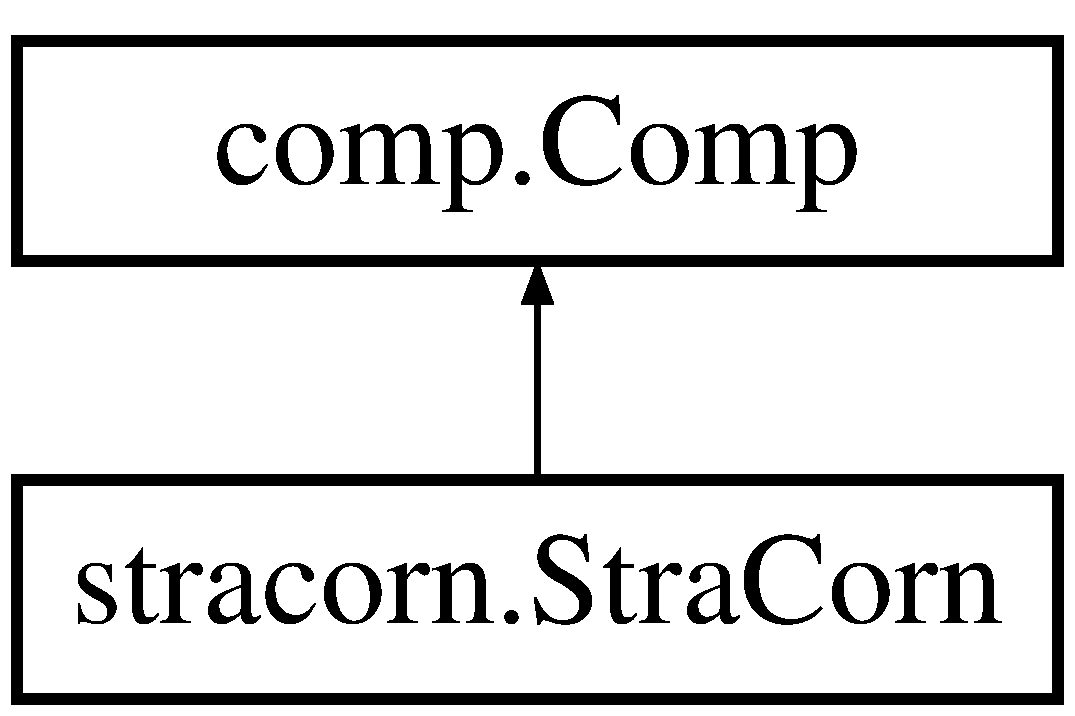
\includegraphics[height=2.000000cm]{classstracorn_1_1StraCorn}
\end{center}
\end{figure}
\subsection*{Public Member Functions}
\begin{DoxyCompactItemize}
\item 
def {\bfseries \+\_\+\+\_\+init\+\_\+\+\_\+} (self, dz\+\_\+dtheta, n\+\_\+layer\+\_\+x, n\+\_\+layer\+\_\+y, offset\+\_\+y, \hyperlink{classcomp_1_1Comp_ae00e132d485d50acaf13977284fd9051}{coord\+\_\+sys}, bdy\+\_\+cond)\hypertarget{classstracorn_1_1StraCorn_a07746366f391cc3a2bc1e30a6f08e221}{}\label{classstracorn_1_1StraCorn_a07746366f391cc3a2bc1e30a6f08e221}

\item 
def \hyperlink{classstracorn_1_1StraCorn_ade20b5300f4291868c5f7fc16d83726c}{create\+Mesh} (self, chem, coord\+\_\+x\+\_\+start, coord\+\_\+y\+\_\+start, water\+\_\+frac\+\_\+surface=.\+55)
\item 
def \hyperlink{classstracorn_1_1StraCorn_ad03208d3f570174098bd28e580ae6ca3}{comp\+Par\+Diff} (self, name, chem, mass\+\_\+frac\+\_\+water, mass\+\_\+frac\+\_\+water\+\_\+sat, V\+\_\+mortar, V\+\_\+brick, V\+\_\+all, T, eta)
\item 
def \hyperlink{classstracorn_1_1StraCorn_aec5858fcc6ac21d7a9051dc34d2ccd18}{comp\+Vol\+Frac\+Water\+\_\+cc} (self, mass\+\_\+frac\+\_\+water, rou\+\_\+lipid, rou\+\_\+keratin, rou\+\_\+water, V\+\_\+mortar\+\_\+geometry, V\+\_\+brick\+\_\+geometry, V\+\_\+all\+\_\+geometry)
\item 
def \hyperlink{classstracorn_1_1StraCorn_ad948bfa716b6245eb4917785e9bc2689}{comp\+O\+D\+Edydt} (self, t, y, args=None)
\item 
def {\bfseries save\+Coord} (self, fn\+\_\+x, fn\+\_\+y)\hypertarget{classstracorn_1_1StraCorn_a76b1184986bb0ce9ad0d514d83f7934c}{}\label{classstracorn_1_1StraCorn_a76b1184986bb0ce9ad0d514d83f7934c}

\end{DoxyCompactItemize}
\subsection*{Public Attributes}
\begin{DoxyCompactItemize}
\item 
{\bfseries w}\hypertarget{classstracorn_1_1StraCorn_a9b85e8b2808dd5dbe759cbdf95df00b1}{}\label{classstracorn_1_1StraCorn_a9b85e8b2808dd5dbe759cbdf95df00b1}

\item 
{\bfseries nx\+\_\+grids\+\_\+lipid}\hypertarget{classstracorn_1_1StraCorn_ae8cccabe0435cfd0dee5ba7d5500c4be}{}\label{classstracorn_1_1StraCorn_ae8cccabe0435cfd0dee5ba7d5500c4be}

\item 
{\bfseries nx\+\_\+grids\+\_\+cc}\hypertarget{classstracorn_1_1StraCorn_a9ee40e138e0ff16bb3b3ec8e8ba9762b}{}\label{classstracorn_1_1StraCorn_a9ee40e138e0ff16bb3b3ec8e8ba9762b}

\item 
{\bfseries ny\+\_\+grids\+\_\+lipid}\hypertarget{classstracorn_1_1StraCorn_acc3a177e7f67c24ff8655a5a836f8e77}{}\label{classstracorn_1_1StraCorn_acc3a177e7f67c24ff8655a5a836f8e77}

\item 
{\bfseries ny\+\_\+grids\+\_\+cc\+\_\+dn}\hypertarget{classstracorn_1_1StraCorn_a45ecced2f8325ebea3782c026dbabbe1}{}\label{classstracorn_1_1StraCorn_a45ecced2f8325ebea3782c026dbabbe1}

\item 
{\bfseries T}\hypertarget{classstracorn_1_1StraCorn_a87f454b2014ff25ac09b55e573d65443}{}\label{classstracorn_1_1StraCorn_a87f454b2014ff25ac09b55e573d65443}

\item 
{\bfseries eta}\hypertarget{classstracorn_1_1StraCorn_aab54cbd9fa36e84970b1ab98ed4f1004}{}\label{classstracorn_1_1StraCorn_aab54cbd9fa36e84970b1ab98ed4f1004}

\item 
{\bfseries geom\+\_\+g}\hypertarget{classstracorn_1_1StraCorn_a87de375fe2dd0451ff04e8326847c6ff}{}\label{classstracorn_1_1StraCorn_a87de375fe2dd0451ff04e8326847c6ff}

\item 
{\bfseries geom\+\_\+d}\hypertarget{classstracorn_1_1StraCorn_a00c555cfc4814339275dbe22b17eef32}{}\label{classstracorn_1_1StraCorn_a00c555cfc4814339275dbe22b17eef32}

\item 
{\bfseries geom\+\_\+s}\hypertarget{classstracorn_1_1StraCorn_a9a736aaf380a1dffa2157337a2c58210}{}\label{classstracorn_1_1StraCorn_a9a736aaf380a1dffa2157337a2c58210}

\item 
{\bfseries geom\+\_\+t}\hypertarget{classstracorn_1_1StraCorn_a13a081cab2aab907a8fba74488300d51}{}\label{classstracorn_1_1StraCorn_a13a081cab2aab907a8fba74488300d51}

\item 
{\bfseries geom\+\_\+dm}\hypertarget{classstracorn_1_1StraCorn_ad83d1ead16e7d8e91100b6f18346b9b7}{}\label{classstracorn_1_1StraCorn_ad83d1ead16e7d8e91100b6f18346b9b7}

\item 
{\bfseries geom\+\_\+dn}\hypertarget{classstracorn_1_1StraCorn_a80e8498d06a7ba4635bacc779bff2cb7}{}\label{classstracorn_1_1StraCorn_a80e8498d06a7ba4635bacc779bff2cb7}

\item 
{\bfseries V\+\_\+mortar}\hypertarget{classstracorn_1_1StraCorn_af85e8a8c4aa005ce418c8164b946a0f5}{}\label{classstracorn_1_1StraCorn_af85e8a8c4aa005ce418c8164b946a0f5}

\item 
{\bfseries V\+\_\+brick}\hypertarget{classstracorn_1_1StraCorn_a5bd0c847e5df8c69a947ed17974cbe3b}{}\label{classstracorn_1_1StraCorn_a5bd0c847e5df8c69a947ed17974cbe3b}

\item 
{\bfseries V\+\_\+all}\hypertarget{classstracorn_1_1StraCorn_ab3dafca0074d669724f20a9c808e0c42}{}\label{classstracorn_1_1StraCorn_ab3dafca0074d669724f20a9c808e0c42}

\item 
{\bfseries offset\+\_\+y}\hypertarget{classstracorn_1_1StraCorn_a6d4f9e4e1897186d86883ab14de4f14c}{}\label{classstracorn_1_1StraCorn_a6d4f9e4e1897186d86883ab14de4f14c}

\item 
{\bfseries meshes}\hypertarget{classstracorn_1_1StraCorn_a298dfda5fde77d782c27f94ee5f4e1ed}{}\label{classstracorn_1_1StraCorn_a298dfda5fde77d782c27f94ee5f4e1ed}

\end{DoxyCompactItemize}


\subsection{Detailed Description}
\begin{DoxyVerb}Class definition for StraCorn, 
which is the stratum corneum, currently modelled as a heterogeneous media
\end{DoxyVerb}
 

Definition at line 17 of file stracorn.\+py.



\subsection{Member Function Documentation}
\index{stracorn\+::\+Stra\+Corn@{stracorn\+::\+Stra\+Corn}!comp\+O\+D\+Edydt@{comp\+O\+D\+Edydt}}
\index{comp\+O\+D\+Edydt@{comp\+O\+D\+Edydt}!stracorn\+::\+Stra\+Corn@{stracorn\+::\+Stra\+Corn}}
\subsubsection[{\texorpdfstring{comp\+O\+D\+Edydt(self, t, y, args=\+None)}{compODEdydt(self, t, y, args=None)}}]{\setlength{\rightskip}{0pt plus 5cm}def stracorn.\+Stra\+Corn.\+comp\+O\+D\+Edydt (
\begin{DoxyParamCaption}
\item[{}]{self, }
\item[{}]{t, }
\item[{}]{y, }
\item[{}]{args = {\ttfamily None}}
\end{DoxyParamCaption}
)}\hypertarget{classstracorn_1_1StraCorn_ad948bfa716b6245eb4917785e9bc2689}{}\label{classstracorn_1_1StraCorn_ad948bfa716b6245eb4917785e9bc2689}
\begin{DoxyVerb}The wrapper function for computing the right hand side of ODEs
\end{DoxyVerb}
 

Definition at line 390 of file stracorn.\+py.

\index{stracorn\+::\+Stra\+Corn@{stracorn\+::\+Stra\+Corn}!comp\+Par\+Diff@{comp\+Par\+Diff}}
\index{comp\+Par\+Diff@{comp\+Par\+Diff}!stracorn\+::\+Stra\+Corn@{stracorn\+::\+Stra\+Corn}}
\subsubsection[{\texorpdfstring{comp\+Par\+Diff(self, name, chem, mass\+\_\+frac\+\_\+water, mass\+\_\+frac\+\_\+water\+\_\+sat, V\+\_\+mortar, V\+\_\+brick, V\+\_\+all, T, eta)}{compParDiff(self, name, chem, mass_frac_water, mass_frac_water_sat, V_mortar, V_brick, V_all, T, eta)}}]{\setlength{\rightskip}{0pt plus 5cm}def stracorn.\+Stra\+Corn.\+comp\+Par\+Diff (
\begin{DoxyParamCaption}
\item[{}]{self, }
\item[{}]{name, }
\item[{}]{chem, }
\item[{}]{mass\+\_\+frac\+\_\+water, }
\item[{}]{mass\+\_\+frac\+\_\+water\+\_\+sat, }
\item[{}]{V\+\_\+mortar, }
\item[{}]{V\+\_\+brick, }
\item[{}]{V\+\_\+all, }
\item[{}]{T, }
\item[{}]{eta}
\end{DoxyParamCaption}
)}\hypertarget{classstracorn_1_1StraCorn_ad03208d3f570174098bd28e580ae6ca3}{}\label{classstracorn_1_1StraCorn_ad03208d3f570174098bd28e580ae6ca3}
\begin{DoxyVerb}Compute the partition coefficient with respect to water
and the diffusion coefficient
\end{DoxyVerb}
 

Definition at line 303 of file stracorn.\+py.

\index{stracorn\+::\+Stra\+Corn@{stracorn\+::\+Stra\+Corn}!comp\+Vol\+Frac\+Water\+\_\+cc@{comp\+Vol\+Frac\+Water\+\_\+cc}}
\index{comp\+Vol\+Frac\+Water\+\_\+cc@{comp\+Vol\+Frac\+Water\+\_\+cc}!stracorn\+::\+Stra\+Corn@{stracorn\+::\+Stra\+Corn}}
\subsubsection[{\texorpdfstring{comp\+Vol\+Frac\+Water\+\_\+cc(self, mass\+\_\+frac\+\_\+water, rou\+\_\+lipid, rou\+\_\+keratin, rou\+\_\+water, V\+\_\+mortar\+\_\+geometry, V\+\_\+brick\+\_\+geometry, V\+\_\+all\+\_\+geometry)}{compVolFracWater_cc(self, mass_frac_water, rou_lipid, rou_keratin, rou_water, V_mortar_geometry, V_brick_geometry, V_all_geometry)}}]{\setlength{\rightskip}{0pt plus 5cm}def stracorn.\+Stra\+Corn.\+comp\+Vol\+Frac\+Water\+\_\+cc (
\begin{DoxyParamCaption}
\item[{}]{self, }
\item[{}]{mass\+\_\+frac\+\_\+water, }
\item[{}]{rou\+\_\+lipid, }
\item[{}]{rou\+\_\+keratin, }
\item[{}]{rou\+\_\+water, }
\item[{}]{V\+\_\+mortar\+\_\+geometry, }
\item[{}]{V\+\_\+brick\+\_\+geometry, }
\item[{}]{V\+\_\+all\+\_\+geometry}
\end{DoxyParamCaption}
)}\hypertarget{classstracorn_1_1StraCorn_aec5858fcc6ac21d7a9051dc34d2ccd18}{}\label{classstracorn_1_1StraCorn_aec5858fcc6ac21d7a9051dc34d2ccd18}
\begin{DoxyVerb}Compute the volume fraction of water in corneocyte
    based on the water content (mass fraction of water) of the stratum corneum
\end{DoxyVerb}
 

Definition at line 367 of file stracorn.\+py.

\index{stracorn\+::\+Stra\+Corn@{stracorn\+::\+Stra\+Corn}!create\+Mesh@{create\+Mesh}}
\index{create\+Mesh@{create\+Mesh}!stracorn\+::\+Stra\+Corn@{stracorn\+::\+Stra\+Corn}}
\subsubsection[{\texorpdfstring{create\+Mesh(self, chem, coord\+\_\+x\+\_\+start, coord\+\_\+y\+\_\+start, water\+\_\+frac\+\_\+surface=.\+55)}{createMesh(self, chem, coord_x_start, coord_y_start, water_frac_surface=.55)}}]{\setlength{\rightskip}{0pt plus 5cm}def stracorn.\+Stra\+Corn.\+create\+Mesh (
\begin{DoxyParamCaption}
\item[{}]{self, }
\item[{}]{chem, }
\item[{}]{coord\+\_\+x\+\_\+start, }
\item[{}]{coord\+\_\+y\+\_\+start, }
\item[{}]{water\+\_\+frac\+\_\+surface = {\ttfamily .55}}
\end{DoxyParamCaption}
)}\hypertarget{classstracorn_1_1StraCorn_ade20b5300f4291868c5f7fc16d83726c}{}\label{classstracorn_1_1StraCorn_ade20b5300f4291868c5f7fc16d83726c}
\begin{DoxyVerb}Create mesh for this compartment
Args:
coord_x_start, coord_y_start: starting coordinates
water_frac_surface : water content (w/w); saturation at .55; dry skin at .25
\end{DoxyVerb}
 

Definition at line 65 of file stracorn.\+py.



The documentation for this class was generated from the following file\+:\begin{DoxyCompactItemize}
\item 
stracorn.\+py\end{DoxyCompactItemize}

\hypertarget{classviaepd_1_1ViaEpd}{}\section{viaepd.\+Via\+Epd Class Reference}
\label{classviaepd_1_1ViaEpd}\index{viaepd.\+Via\+Epd@{viaepd.\+Via\+Epd}}
Inheritance diagram for viaepd.\+Via\+Epd\+:\begin{figure}[H]
\begin{center}
\leavevmode
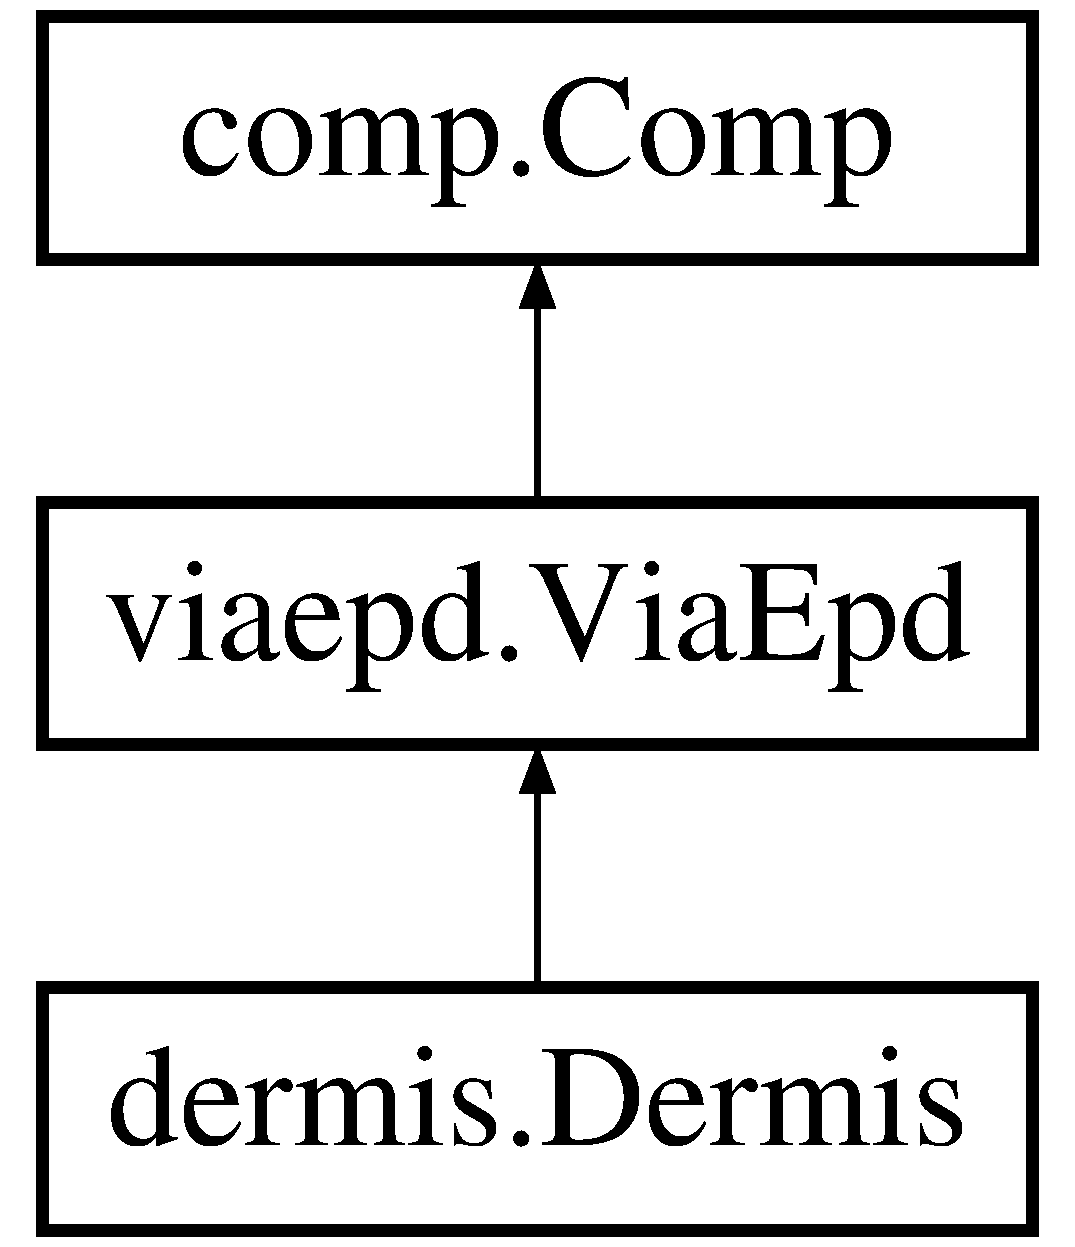
\includegraphics[height=2.000000cm]{classviaepd_1_1ViaEpd}
\end{center}
\end{figure}
\subsection*{Public Member Functions}
\begin{DoxyCompactItemize}
\item 
def {\bfseries \+\_\+\+\_\+init\+\_\+\+\_\+} (self, \hyperlink{classcomp_1_1Comp_ae00e132d485d50acaf13977284fd9051}{coord\+\_\+sys}=None, dz\+\_\+dtheta=None, bdy\+\_\+cond=None)\hypertarget{classviaepd_1_1ViaEpd_a366b3abf6268874ec0a38a0927e6e030}{}\label{classviaepd_1_1ViaEpd_a366b3abf6268874ec0a38a0927e6e030}

\item 
def \hyperlink{classviaepd_1_1ViaEpd_aca401fb9bc87b50c59ef25b157227727}{create\+Mesh} (self, chem, coord\+\_\+x\+\_\+start, coord\+\_\+y\+\_\+start)
\item 
def \hyperlink{classviaepd_1_1ViaEpd_ac206abcf43729b9906dc75cbd49283fe}{comp\+Par\+Diff} (self, chem)
\item 
def {\bfseries save\+Coord} (self, fn\+\_\+x, fn\+\_\+y)\hypertarget{classviaepd_1_1ViaEpd_a99b4ca36f663b30b87a13a51b9b62776}{}\label{classviaepd_1_1ViaEpd_a99b4ca36f663b30b87a13a51b9b62776}

\end{DoxyCompactItemize}
\subsection*{Public Attributes}
\begin{DoxyCompactItemize}
\item 
{\bfseries Kw}\hypertarget{classviaepd_1_1ViaEpd_a0a4894a612c4d045d872ccf1fb674578}{}\label{classviaepd_1_1ViaEpd_a0a4894a612c4d045d872ccf1fb674578}

\item 
{\bfseries D}\hypertarget{classviaepd_1_1ViaEpd_aa552bd94144bb3b0984127f446c15dd6}{}\label{classviaepd_1_1ViaEpd_aa552bd94144bb3b0984127f446c15dd6}

\item 
{\bfseries meshes}\hypertarget{classviaepd_1_1ViaEpd_a4f929b4abcbb79bb340237db65b9b33b}{}\label{classviaepd_1_1ViaEpd_a4f929b4abcbb79bb340237db65b9b33b}

\end{DoxyCompactItemize}


\subsection{Detailed Description}
\begin{DoxyVerb}Class definition for ViaEpd
which is the viable epidermis, currently modelled as a homogenised media
\end{DoxyVerb}
 

Definition at line 14 of file viaepd.\+py.



\subsection{Member Function Documentation}
\index{viaepd\+::\+Via\+Epd@{viaepd\+::\+Via\+Epd}!comp\+Par\+Diff@{comp\+Par\+Diff}}
\index{comp\+Par\+Diff@{comp\+Par\+Diff}!viaepd\+::\+Via\+Epd@{viaepd\+::\+Via\+Epd}}
\subsubsection[{\texorpdfstring{comp\+Par\+Diff(self, chem)}{compParDiff(self, chem)}}]{\setlength{\rightskip}{0pt plus 5cm}def viaepd.\+Via\+Epd.\+comp\+Par\+Diff (
\begin{DoxyParamCaption}
\item[{}]{self, }
\item[{}]{chem}
\end{DoxyParamCaption}
)}\hypertarget{classviaepd_1_1ViaEpd_ac206abcf43729b9906dc75cbd49283fe}{}\label{classviaepd_1_1ViaEpd_ac206abcf43729b9906dc75cbd49283fe}
\begin{DoxyVerb}Compute the partition coefficient with respect to water
and the diffusion coefficient
\end{DoxyVerb}
 

Definition at line 64 of file viaepd.\+py.

\index{viaepd\+::\+Via\+Epd@{viaepd\+::\+Via\+Epd}!create\+Mesh@{create\+Mesh}}
\index{create\+Mesh@{create\+Mesh}!viaepd\+::\+Via\+Epd@{viaepd\+::\+Via\+Epd}}
\subsubsection[{\texorpdfstring{create\+Mesh(self, chem, coord\+\_\+x\+\_\+start, coord\+\_\+y\+\_\+start)}{createMesh(self, chem, coord_x_start, coord_y_start)}}]{\setlength{\rightskip}{0pt plus 5cm}def viaepd.\+Via\+Epd.\+create\+Mesh (
\begin{DoxyParamCaption}
\item[{}]{self, }
\item[{}]{chem, }
\item[{}]{coord\+\_\+x\+\_\+start, }
\item[{}]{coord\+\_\+y\+\_\+start}
\end{DoxyParamCaption}
)}\hypertarget{classviaepd_1_1ViaEpd_aca401fb9bc87b50c59ef25b157227727}{}\label{classviaepd_1_1ViaEpd_aca401fb9bc87b50c59ef25b157227727}
\begin{DoxyVerb}Create mesh for this compartment
Args:
coord_x_start, coord_y_start: starting coordinates
\end{DoxyVerb}
 

Definition at line 27 of file viaepd.\+py.



The documentation for this class was generated from the following file\+:\begin{DoxyCompactItemize}
\item 
viaepd.\+py\end{DoxyCompactItemize}

%--- End generated contents ---

% Index
\backmatter
\newpage
\phantomsection
\clearemptydoublepage
\addcontentsline{toc}{chapter}{Index}
\printindex

\end{document}
